% This is samplepaper.tex, a sample chapter demonstrating the
% LLNCS macro package for Springer Computer Science proceedings;
% Version 2.20 of 2017/10/04
%
\documentclass[runningheads]{llncs}
%
\usepackage{graphicx}
% Used for displaying a sample figure. If possible, figure files should
% be included in EPS format.
%
% If you use the hyperref package, please uncomment the following line
% to display URLs in blue roman font according to Springer's eBook style:
% \renewcommand\UrlFont{\color{blue}\rmfamily}
\usepackage[misc,geometry]{ifsym}
\usepackage{graphicx}
\usepackage{multirow}
\usepackage{algorithm}
\usepackage{algorithmic}
% \usepackage{algpseudocode}
\usepackage{makecell}
\usepackage{tabularx}
\usepackage{multirow}
\usepackage{amsmath}
\usepackage{xcolor}
\usepackage{blkarray, bigstrut}
\usepackage{hyperref}
\hypersetup{colorlinks=true,citecolor=blue}
\usepackage{amsfonts}
\usepackage{siunitx}
\usepackage{dsfont}
\usepackage{lipsum}
\usepackage{adjustbox}
\usepackage{float}
\usepackage{booktabs}
\usepackage{cite}
\usepackage{bm}
\usepackage{pifont}
\usepackage{relsize}

\newcommand\eg {{\it e.g., }}
\newcommand\st {{\it s.t., }}
\newcommand{\cmark}{\ding{51}}%
\newcommand{\xmark}{\ding{55}}%
\newcommand*\rot{\rotatebox{90}}
\newcommand*\OK{\ding{51}}
\newcommand\ie {{\it i.e., }}
\newcommand*\mystrut[1]{\vrule width0pt height0pt depth#1\relax}
\begin{document}
%
\title{
Distilling BlackBox to Interpretable models for Efficient Transfer Learning
% Interpretable Model Distillation for Efficient Transfer Learning
% Efficient Transfer Learning via Distillation of Interpretable Neural Networks
}
%
%\titlerunning{Abbreviated paper title}
% If the paper title is too long for the running head, you can set
% an abbreviated paper title here
%
\author{Shantanu Ghosh\inst{1}{$^{(\textrm{\Letter})}$}\and
Ke Yu\inst{2}\and
Kayhan Batmanghelich\inst{1}}

\authorrunning{S. Ghosh et al.}
% First names are abbreviated in the running head.
% If there are more than two authors, 'et al.' is used.
%
\institute{
Department of Electrical and Computer Engineering, Boston University, Boston, MA, USA \\
\email{shawn24@bu.edu}\\
\and
Intelligent Systems Program, University of Pittsburgh, Pittsburgh, PA, USA 
}


%
\maketitle              % typeset the header of the contribution
%
\begin{abstract}
    Building generalizable AI models is one of the primary challenges in the healthcare domain.
While radiologists rely on generalizable descriptive rules of abnormality, Neural Network (NN) models suffer even with a slight shift in input distribution (\eg scanner type).
Fine-tuning a model to transfer knowledge from one domain to another requires a significant amount of labeled data in the target domain. 
In this paper, we develop an interpretable model that can be efficiently fine-tuned to an unseen target domain with minimal computational cost.
We assume the interpretable component of NN to be approximately domain-invariant.
However, interpretable models typically underperform compared to their Blackbox (BB) variants. We start with a BB in the source domain and distill it into a \emph{mixture} of shallow interpretable models using human-understandable concepts. 
As each interpretable model covers a subset of data, a mixture of interpretable models achieves comparable performance as BB.
Further, we use the pseudo-labeling technique from semi-supervised learning (SSL) to learn the concept classifier in the target domain, followed by fine-tuning the interpretable models in the target domain.
We evaluate our model using a real-life large-scale chest-X-ray (CXR) classification dataset.
The code is available at: \url{https://github.com/batmanlab/MICCAI-2023-Route-interpret-repeat-CXRs}.
    \keywords{
        Explainable-AI \and
        Interpretable models \and
        Transfer learning
    }
\end{abstract}

% Developing a generalizable model is one of the main challenges of AI in the healthcare domain
% While radiologists rely on descriptive explanations of abnormality which are fairly generalizable, DL models struggle even by the smaller shift in the distribution of input (eg scanner type)
% Developing a data-efficient transfer learning can alleviate this problem
% Currently, transfer learning from one to another domain requires a substantial amount of label data in the target domain
% In this paper, we develop an interpretable model that can be efficiently transferred between two domains
% The idea is that the interpretable part of a model is approximately invariant between domains
% However,  interpretable models usually underperform the blackbox models. We address this issue by starting from a blackbox model and gradually distill the blackbox to a mixture of interpretable models. Our approach yields a mixture of interptrable models applied on the concept level that does not compromise in performance.
% During the transfer, we apply pseduo label semi-supervised learning technique to adjust and concept classifier, then fine-tune a shallow interpretable model.
% We evaluate our model on classification problems on several chest X-ray classification datasets.
%
%
\section{Introduction}
Model generalizability is one of the main challenges of AI, especially in high stake applications such as healthcare. While NN models achieve state-of-the-art (SOTA) performance in disease classification~\cite{irvin2019chexpert, rajpurkar2017chexnet, yu2022anatomy}, they are brittle to small shifts in the data distribution~\cite{guan2021domain} caused by a change in acquisition protocol or scanner type~\cite{yan2020mri}. Fine-tuning all or some layers of a NN model on the target domain can alleviate this problem~\cite{chu2016best}, but it requires a substantial amount of labeled data and be computationally expensive~\cite{wang2017growing, kandel2020deeply}. In contrast, radiologists follow fairly generalizable and comprehensible rules. Specifically, they search for patterns of changes in anatomy to read abnormality from an image and apply logical rules for specific diagnoses. This approach is transparent and closer to an interpretable-by-design approach in AI. We develop a method to extract a mixture of interpretable models based on clinical concepts, similar to radiologists' rules, from a pre-trained NN. Such a model is more data- and computation-efficient than the original NN for fine-tuning to a new distribution.

 Standard interpretable by design method~\cite{rudin2022interpretable} finds an interpretable function (\eg linear regression or rule-based) between human-interpretable concepts and final output~\cite{koh2020concept}. A concept classifier~\cite{sarkar2021inducing, zarlenga2022concept} detects the presence or absence of concepts in an image. In medical images, previous research uses TCAV scores~\cite{kim2017interpretability} to quantify the role of a concept on the final prediction~\cite{yeche2019ubs, graziani2020concept, clough2019global}, but the concept-based interpretable models have been mostly unexplored.
% and used for medical imaging purposes~\cite{yeche2019ubs, graziani2020concept, clough2019global}. 
Recently Posthoc Concept Bottleneck models (PCBMs)~\cite{yuksekgonul2022post} identify concepts from the embeddings of BB. However, the common design choice amongst those methods relies on a single interpretable classifier to explain the entire dataset, cannot capture the diverse sample-specific explanations, and performs poorly than their BB variants.

\textbf{Our contributions.}
This paper proposes a novel data-efficient interpretable method that can be transferred to an unseen domain. Our interpretable model is built upon human-interpretable concepts and can provide sample-specific explanations for diverse disease subtypes and pathological patterns. Beginning with a BB in the source domain, we progressively extract a mixture of interpretable models from BB. Our method includes a set of selectors routing the explainable samples through the interpretable models. The interpretable models provide First-order-logic (FOL) explanations for the samples they cover. The remaining unexplained samples are routed through the residuals until they are covered by a successive interpretable model. We repeat the process until we cover a desired fraction of data. Due to class imbalance in large CXR datasets, early interpretable models tend to cover all samples with disease present while ignoring disease subgroups and pathological heterogeneity. We address this problem by estimating the class-stratified coverage from the total data coverage. We then finetune the interpretable models in the target domain. The target domain lacks concept-level annotation since they are expensive. Hence, we learn a concept detector in the target domain with a pseudo labeling approach~\cite{lee2013pseudo} and finetune the interpretable models. Our work is the first to apply concept-based methods to CXRs and transfer them between domains. 

% Our experiments demonstrate that our method (1) is able to capture diverse instance-specific concepts in the FOL explanations compared to all other interpretable models, (2) does not compromise the performance, (3) is able to identify ``harder'' samples, (4) can be efficiently transferred from source to target domain.
 

\label{sec:intro}

% \section{Background: Route, Interpret, and Repeat}
% Assume $f^0: \mathcal{X} \rightarrow \mathcal{Y}$ is a BB, trained on a dataset \{$\mathcal{X}$, $\mathcal{Y}$, $\mathcal{C}$\}, with $\mathcal{X}$, $\mathcal{Y}$, and $\mathcal{C}$ being the images, classes, and human interpretable concepts, respectively. Further, $f^0=h^0 \circ \Phi$. Given a learnable projection $t: \Phi \rightarrow \mathcal{C}$, the iterative algorithm \emph{Route, Interpret, and Repeat (RIR)}~\cite{ghosh2023route} carves out an interpretable expert ($g^k: \mathcal{C} \rightarrow \mathcal{Y}$) and a residual ($r^k :\Phi\rightarrow\mathcal{Y}$) at each iteration $k$, explaining the interpretable and uninterpretable components of $f^0$ respectively. Each expert specializes in a subset of data, defined by that iteration's coverage $\tau^k$. 
The algorithm learns three functions: (1) a set of probabilistic selectors \emph{routing} a sample to the corresponding expert or the residual, (2) a set of experts, each generating sample-specific FOLs in terms of the concepts to \emph{interpret} the BB, and (3) \emph{repeating} with residuals for the unexplained samples.



% \label{sec:background}

\section{Methodology}
%
\textbf{Notation and learning the concepts:} 
Assume $f^0: \mathcal{X} \rightarrow \mathcal{Y}$ is a pre-trained Blackbox predicting the output from the input image. Also, $\displaystyle f^0(.) =  h^0 \circ \Phi(.) $. Here, $ \Phi: \mathcal{X} \rightarrow R^l $ is the image embeddings and $ h^0: R^l \rightarrow \mathcal{Y}$ is the classifier, classifying the output $\mathcal{Y}$ using the embeddings, $\Phi$. Our approach is applicable for both datasets with and without human-interpretable concept annotations. For datasets with the concept annotation $\mathcal{C} \in \mathbb{R}^{N_c}$ ($N_c$ being the number of concepts per image $\mathcal{X}$), we learn $t: R^l \rightarrow\mathcal{C}$ to classify the concepts using the embeddings. Per this definition, $t$ outputs a scalar value $c$ representing a single concept for each input image. 
%We adopt the concept learning strategy in PosthocCBM (PCBM)~\cite{yuksekgonul2022post} for datasets without concept annotation. 
%Specifically, we leverage a set of image embeddings with the concept being present and absent. Next, we learn a linear SVM to construct the concept activation matrix~\cite{kim2017interpretability} as $\boldsymbol{Q} \in\mathbb{R}^{N_c \times l}$. 
Finally we estimate the concept value as $c = \frac{<\Phi(x), q^i>}{||q_i||_2^2}$ $ \in \mathbb{R}$ utilizing each row $\boldsymbol{q^i}$ of $\boldsymbol{Q}$. Thus, the complete tuple of $j^{th}$ sample is $\{x_j, y_j, c_j\}$, denoting the image, label, and learned concept vector, respectively.

\textbf{Method Overview:} 
Figure \ref{fig:Schematic} summarizes our approach. We iteratively carve out an interpretable model from the given Blackbox. Each iteration yields an interpretable model (the downward grey paths in Figure \ref{fig:Schematic}) and a residual (the straightforward black paths in Figure \ref{fig:Schematic}).
We start with the initial Blackbox $f^0$.
At iteration $k$, we distill the Blackbox from the previous iteration $f^{k-1}$ into a neuro-symbolic interpretable model, $\displaystyle g^{k}: \mathcal{C} \rightarrow \mathcal{Y}$. Our $g$ is flexible enough to be any interpretable models \eg logistic classifier~\cite{yuksekgonul2022post, koh2020concept, barbiero2022entropy}. The \emph{residual} $r^k =f^{k-1} - g^k$ emphasizes the portion of $f^{k-1}$ that $g^k$cannot explain. We then approximate $r^k$ with $f^{k} = h^k(\Phi(.))$. $f^k$ will be the Blackbox for the subsequent iterations and be explained by the respective interpretable model. 
% Due to computational reasons, we only finetune $h^{k}$ to optimize for $r^k$. 
A learnable gating mechanism, denoted by $\pi^k : \mathcal{C} \rightarrow \{0,1\}$ (shown as the \emph{selector} in figure \ref{fig:Schematic}) routes an input sample towards either $g^k$ or $r^k$.
% In order to learn $\pi^k$, we use simple backpropagation while learning $g^k$. A
The thickness of the lines in Figure \ref{fig:Schematic} represents the samples covered by the interpretable models (grey line) and the residuals (black line). 
% Our method is designed such that it leaves a little number of samples for the last residual blackbox.
With every iteration, the cumulative coverage of the interpretable models increases, but the residual decreases. We name our method \emph{route, interpret} and \emph{repeat}.

\subsection{Neuro-Symbolic Knowledge Distillation}
Knowledge distillation in our method involves 3 parts: (1) a series of trainable selectors ,\emph{routing} each sample through the interpretable models and the residual networks, (2) A sequence of learnable neuro-symbolic interpretable models, each providing FOL explanations to \emph {interpret} the Blackbox, and (3) \emph{repeating} with Residuals for the samples that cannot be explained with their interpretable counterparts. 
We detail each component below.

\begin{figure}[h]
% \vskip 0.2in
\centering
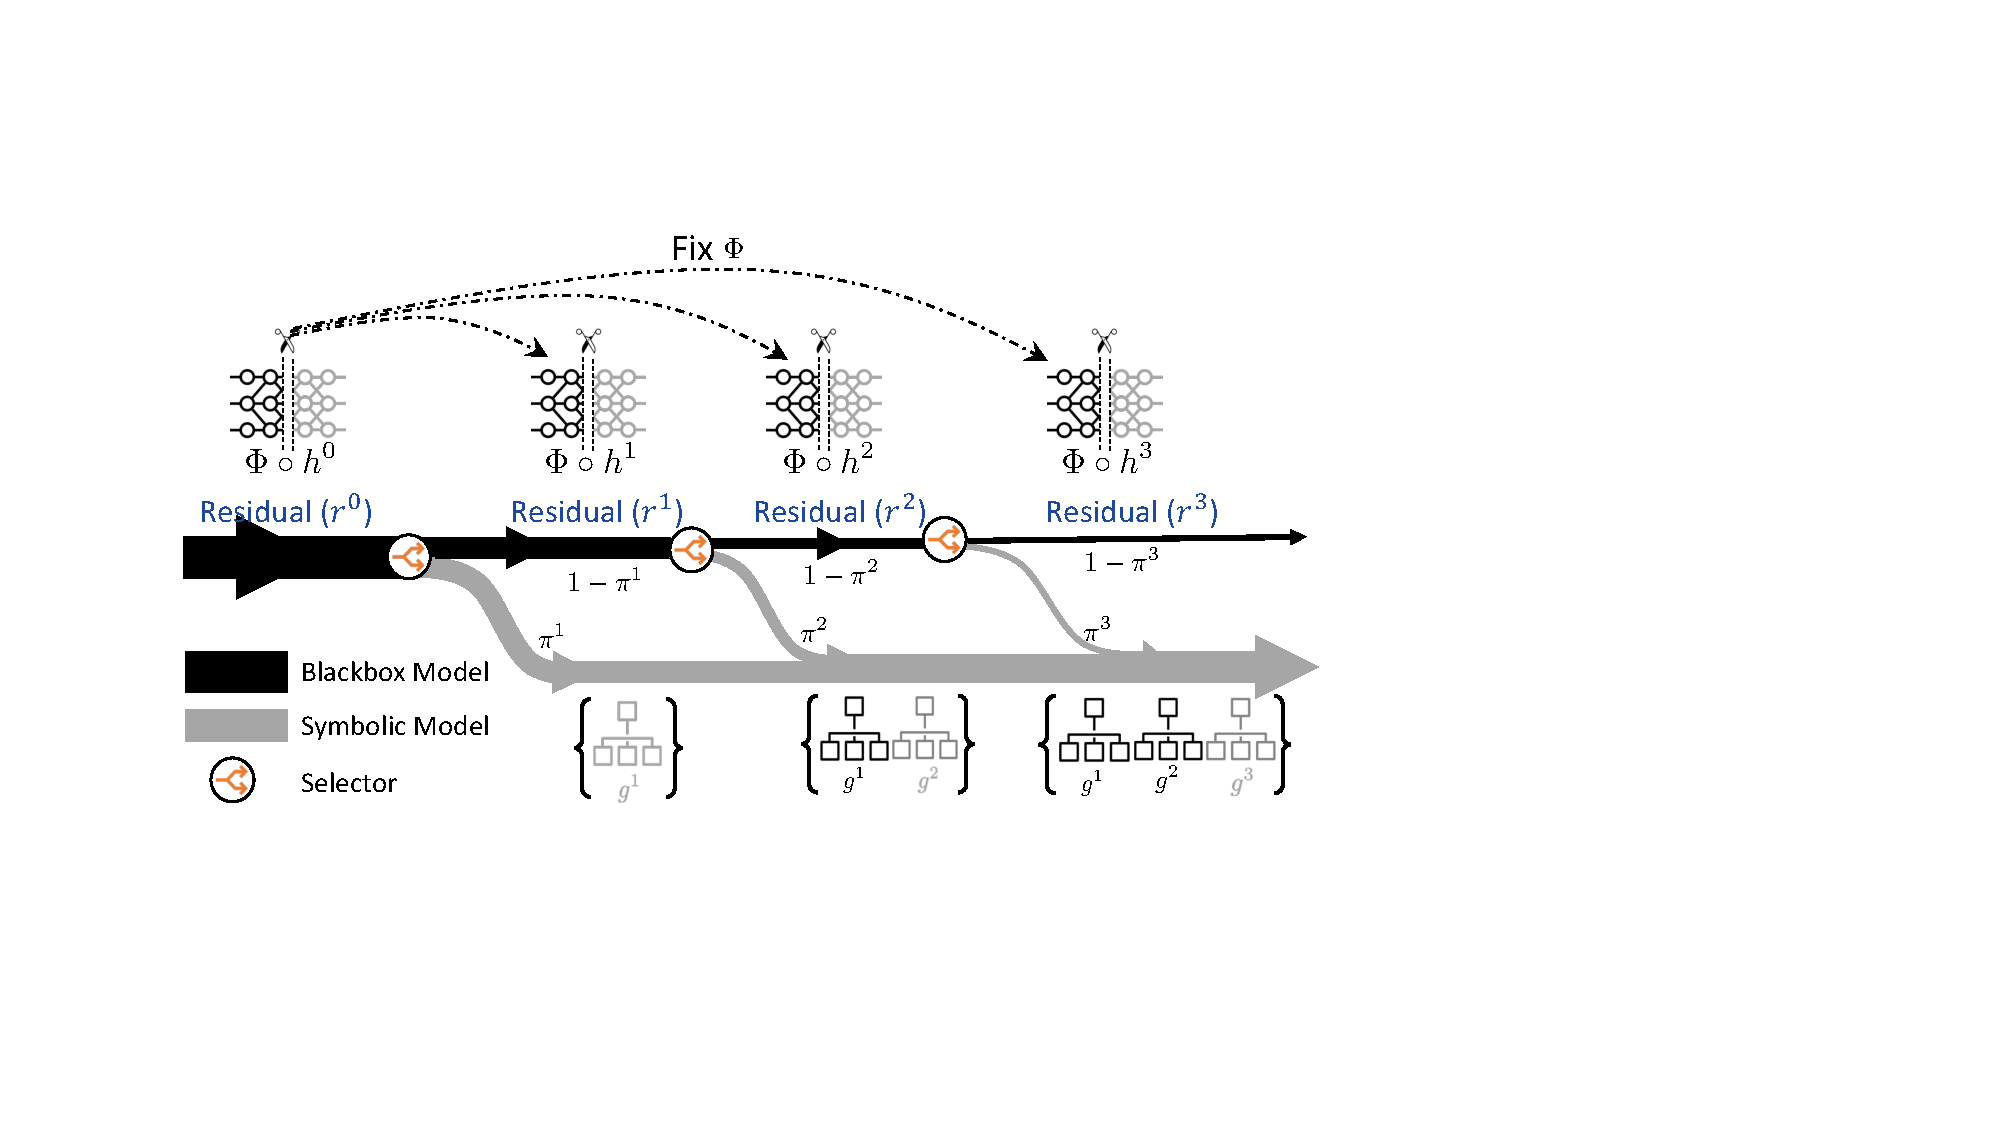
\includegraphics[width=\columnwidth]{figures/main/schematic.pdf}
\vskip -3pt
\caption{Schematic view of \emph{route, interpret} and \emph{repeat}. At iteration $k$, the selector \emph{routes} each sample either towards the interpretable model $g^k$ (to \emph{interpret}) with probability $\pi^k(.)$ or the residual $r^k = f^{k-1} - g^k$ with probability $1-\pi^k(.)$ (to \emph{repeat} in the further iterations). $f^{k-1}$ is the Blackbox of the $(k-1)^{th}$ iteration. $g^k$ generates FOL-based explanations for the samples it covers. Otherwise, the selector routes through the next step until it either goes through a subsequent interpretable model or reaches the last residual. Also, components in black and grey indicate the fixed and trainable modules in our model respectively. }
\label{fig:Schematic} 
\vskip -0.1in
\end{figure}

\subsubsection{The selector function}
As the first step of our method, the selector $\pi^k$ \emph{routes} the $j^{th}$ sample through the interpretable model $g^k$ or residual $r^k$ with probability $\displaystyle \pi^k(\boldsymbol{c_j})$ and $\displaystyle 1 - \pi^k(\boldsymbol{c_j})$ respectively, where $k$ $\in [0,K]$, with $K$ being the number of iterations.
We define the empirical coverage of the $\displaystyle k^{th}$ iteration as $\vspace{-0.08pt} \zeta(\pi^k) = \frac{1}{m}\sum_{j = 1} ^ m \pi^k(\boldsymbol{c_j}) \vspace{-0.081pt}$, the empirical mean of the samples selected by the selector for the associated interpretable model $\displaystyle g^k$, with $\displaystyle m$ being the total number of samples in the training set. Thus, the entire selective risk is:

\vskip -7.5pt
\begin{equation}
\label{equ: emp_risk}
\mathcal{R}^k(\displaystyle \pi^k, \displaystyle g^k) = \frac{\frac{1}{m}\sum_{j=1}^m\mathcal{L}_{(g^k, \pi^k)}^k\big(\boldsymbol{x_j}, \boldsymbol{c_j}\big)}{\zeta(\pi^k)} ,
\end{equation}
\vskip 2pt

where $\mathcal{L}_{(g^k, \pi^k)}^k$ is the optimization loss used to learn $\displaystyle g^k$ and $\displaystyle \pi^k$ together, discussed in section \ref{ns-optimization}. For a given coverage of $\displaystyle \tau^k \in (0, 1]$, we solve the following optimization problem:

\vskip -7.5pt
\begin{align}
\label{equ: optimization_g}
\theta_{s^k}^*, \theta_{g^k}^* = & \operatorname*{arg\,min}_{\theta_{s^k}, \theta_{g^k}} \mathcal{R}^k\Big(\pi^k(.; \theta_{s^k}), \displaystyle g^k(.; \theta_{g^k}) \Big) \nonumber \\ 
&\text{s.t.} ~~~ \zeta\big(\pi^k(.; \theta_{s^k})\big) \geq \tau^k,
\end{align}
\vskip 2pt

where $\theta_{s^k}^*, \theta_{g^k}^*$ are the optimal parameters at iteration $k$ for the selector $\pi^k$ and the interpretable model $g^k$ respectively. In this work, $\pi$s' of different iterations are neural networks with sigmoid activation. At inference time, the selector routes the $j^{th}$ sample with concept vector $\boldsymbol{c_j}$ to $\displaystyle g^k$ if and only if $\pi^k(\boldsymbol{c}_j)\geq 0.5$ for $k \in [0,K]$.

\subsubsection{Neuro-Symbolic interpretable models}
\label{ns-optimization}
In this stage, we design interpretable model $\displaystyle g^k$ of $k^{th}$ iteration  to \emph{interpret} the Blackbox $\displaystyle f^{k - 1}$ from the previous $(k-1)^{th}$ iteration by optimizing the following loss function:
\begin{equation}
\label{equ: g_k}
\resizebox{0.47\textwidth}{!}{$
\mathcal{L}_{(g^k, \pi^k)}^k\big(\boldsymbol{x_j}, \boldsymbol{c_j}\big) = \underbrace{\mystrut{2.6ex}\ell\Big(f^{k - 1}(\boldsymbol{x_j}), g^k(\boldsymbol{c_j})\Big)\pi^k(c_j) }_{\substack{\text{trainable component} \\ \text{for current iteration $k$}}}\underbrace{\prod_{i=1} ^{k - 1}\big(1 - \pi^i(\boldsymbol{c_j})\big)}_{\substack{\text{fixed component trained} \\ \text{in the previous iterations}}},
$}
\end{equation}

where the term $\pi^k(\boldsymbol{c_j})\prod_{i=1} ^{k - 1}\big(1 - \pi^i(\boldsymbol{c_j}) \big)$ denotes the probability of $j^{th}$ sample being routed through the interpretable model $g^k$. It is the probability of the sample going through the residuals for all the previous iterations from $0$ through $k-1$ (\ie $\prod_{i=1} ^{k - 1}\big(1 - \pi^i(\boldsymbol{c_j}) \big)$\big) times the probability of going through the interpretable model at iteration $k$ \big(\ie $\pi^k(\boldsymbol{c_j})$\big). 
Refer to Figure~\ref{fig:Schematic} for an illustration. We learn $\pi^1, \dots \pi^{k - 1}$ in the prior iterations and are not trainable at iteration $k$. As each interpretable model $g^k$ specializes in explaining a specific subset of samples (denoted by coverage $\tau$), we refer to it as an \emph{expert}. We use SelectiveNet's ~\cite{geifman2019selectivenet}  optimization method to optimize equation \ref{equ: optimization_g} since selectors need a rejection mechanism to route samples through residuals. Appendix \ref{app:loss} details the optimization procedure in equation \ref{equ: g_k}. We refer to the interpretable experts of all the iterations as a ``Mixture of Interpretable Experts'' (MoIE) cumulatively after training. Furthermore, we utilize Entropy-based linear layer neural network (ELL)~\cite{barbiero2022entropy} as the interpretable symbolic model $g$ to construct First Order Logic (FOL) explanations of a given prediction.

\subsubsection{The Residuals}
The last step is to \emph{repeat} with the residual $r^k$, as $\displaystyle r^k(\boldsymbol{x_j},\boldsymbol{c_j}) = f^{k - 1}(\boldsymbol{x_j}) - g^k(\boldsymbol{c_j})$.
We train $f^k = h^k\big(\Phi(.)\big)$ to approximate the residual $r^k$, creating a new Blackbox $f^k$ for the next iteration $(k+1$). This step is necessary to specialize $\displaystyle f^k$ over samples not covered by $g^k$. Optimizing the following loss function yields $\displaystyle f^k$ for the $\displaystyle k^{th}$ iteration:
\begin{equation}
\label{equ: residual}
\mathcal{L}_f^k(\boldsymbol{x_j}, \boldsymbol{c_j}) = \underbrace{\mystrut{2.6ex}\ell\big(r^k(\boldsymbol{x_j}, \boldsymbol{c_j}), f^k(\boldsymbol{x_j})\big)}_{\substack{\text{trainable component} \\ \text{for iteration $k$}}} \underbrace{\mystrut{2.6ex}\prod_{i=1} ^{k}\big(1 - \pi^i(\boldsymbol{c_j})\big)}_{\substack{\text{non-trainable component} \\ \text{for iteration $k$}}} 
\end{equation}

% \underbrace{\mystrut{2.6ex}\ell\big(f^{k - 1}(\boldsymbol{x_j}), g^k(\boldsymbol{c_j})\big)\pi^k(c_j) }_{\substack{\text{trainable component} \\ \text{from current iteration}}}
Notice that we fix the embedding $\displaystyle \Phi(.)$ for all the iterations. Due to computational overhead, we only finetune the last few layers of the Blackbox ($h^k$) to train $f^k$.
At the final iteration $K$, our method produces a MoIE and a Residual, explaining the interpretable and uninterpretable components of the initial Blackbox $f^0$, respectively. Appendix \ref{app:algo} describes the training procedure of our model, the extraction of FOL and the architecture of our model at inference.


\textbf{Selecting number of iterations $K$:} We follow two principles to select the number of iterations $K$ as a stopping criterion: 1) Each expert should have enough data to be trained reliably (
coverage $\zeta^k$). If an expert covers insufficient samples, we stop the process. 2) If the final residual ($r^K$) underperforms a threshold, it is not reliable to distill from the Blackbox. We stop the procedure to ensure the overall accuracy is maintained.

\textbf{Notation and learning the concepts:} 
Assume $f^0: \mathcal{X} \rightarrow \mathcal{Y}$ is a pre-trained Blackbox predicting the output from the input image. Also, $\displaystyle f^0(.) =  h^0 \circ \Phi(.) $. Here, $ \Phi: \mathcal{X} \rightarrow R^l $ is the image embeddings and $ h^0: R^l \rightarrow \mathcal{Y}$ is the classifier, classifying the output $\mathcal{Y}$ using the embeddings, $\Phi$. Our approach is applicable for both datasets with and without human-interpretable concept annotations. For datasets with the concept annotation $\mathcal{C} \in \mathbb{R}^{N_c}$ ($N_c$ being the number of concepts per image $\mathcal{X}$), we learn $t: R^l \rightarrow\mathcal{C}$ to classify the concepts using the embeddings. Per this definition, $t$ outputs a scalar value $c$ representing a single concept for each input image. 
%We adopt the concept learning strategy in PosthocCBM (PCBM)~\cite{yuksekgonul2022post} for datasets without concept annotation. 
%Specifically, we leverage a set of image embeddings with the concept being present and absent. Next, we learn a linear SVM to construct the concept activation matrix~\cite{kim2017interpretability} as $\boldsymbol{Q} \in\mathbb{R}^{N_c \times l}$. 
Finally we estimate the concept value as $c = \frac{<\Phi(x), q^i>}{||q_i||_2^2}$ $ \in \mathbb{R}$ utilizing each row $\boldsymbol{q^i}$ of $\boldsymbol{Q}$. Thus, the complete tuple of $j^{th}$ sample is $\{x_j, y_j, c_j\}$, denoting the image, label, and learned concept vector, respectively.

\textbf{Method Overview:} 
Figure \ref{fig:Schematic} summarizes our approach. We iteratively carve out an interpretable model from the given Blackbox. Each iteration yields an interpretable model (the downward grey paths in Figure \ref{fig:Schematic}) and a residual (the straightforward black paths in Figure \ref{fig:Schematic}).
We start with the initial Blackbox $f^0$.
At iteration $k$, we distill the Blackbox from the previous iteration $f^{k-1}$ into a neuro-symbolic interpretable model, $\displaystyle g^{k}: \mathcal{C} \rightarrow \mathcal{Y}$. Our $g$ is flexible enough to be any interpretable models \eg logistic classifier~\cite{yuksekgonul2022post, koh2020concept, barbiero2022entropy}. The \emph{residual} $r^k =f^{k-1} - g^k$ emphasizes the portion of $f^{k-1}$ that $g^k$cannot explain. We then approximate $r^k$ with $f^{k} = h^k(\Phi(.))$. $f^k$ will be the Blackbox for the subsequent iterations and be explained by the respective interpretable model. 
% Due to computational reasons, we only finetune $h^{k}$ to optimize for $r^k$. 
A learnable gating mechanism, denoted by $\pi^k : \mathcal{C} \rightarrow \{0,1\}$ (shown as the \emph{selector} in figure \ref{fig:Schematic}) routes an input sample towards either $g^k$ or $r^k$.
% In order to learn $\pi^k$, we use simple backpropagation while learning $g^k$. A
The thickness of the lines in Figure \ref{fig:Schematic} represents the samples covered by the interpretable models (grey line) and the residuals (black line). 
% Our method is designed such that it leaves a little number of samples for the last residual blackbox.
With every iteration, the cumulative coverage of the interpretable models increases, but the residual decreases. We name our method \emph{route, interpret} and \emph{repeat}.

\subsection{Neuro-Symbolic Knowledge Distillation}
Knowledge distillation in our method involves 3 parts: (1) a series of trainable selectors ,\emph{routing} each sample through the interpretable models and the residual networks, (2) A sequence of learnable neuro-symbolic interpretable models, each providing FOL explanations to \emph {interpret} the Blackbox, and (3) \emph{repeating} with Residuals for the samples that cannot be explained with their interpretable counterparts. 
We detail each component below.

\begin{figure}[h]
% \vskip 0.2in
\centering
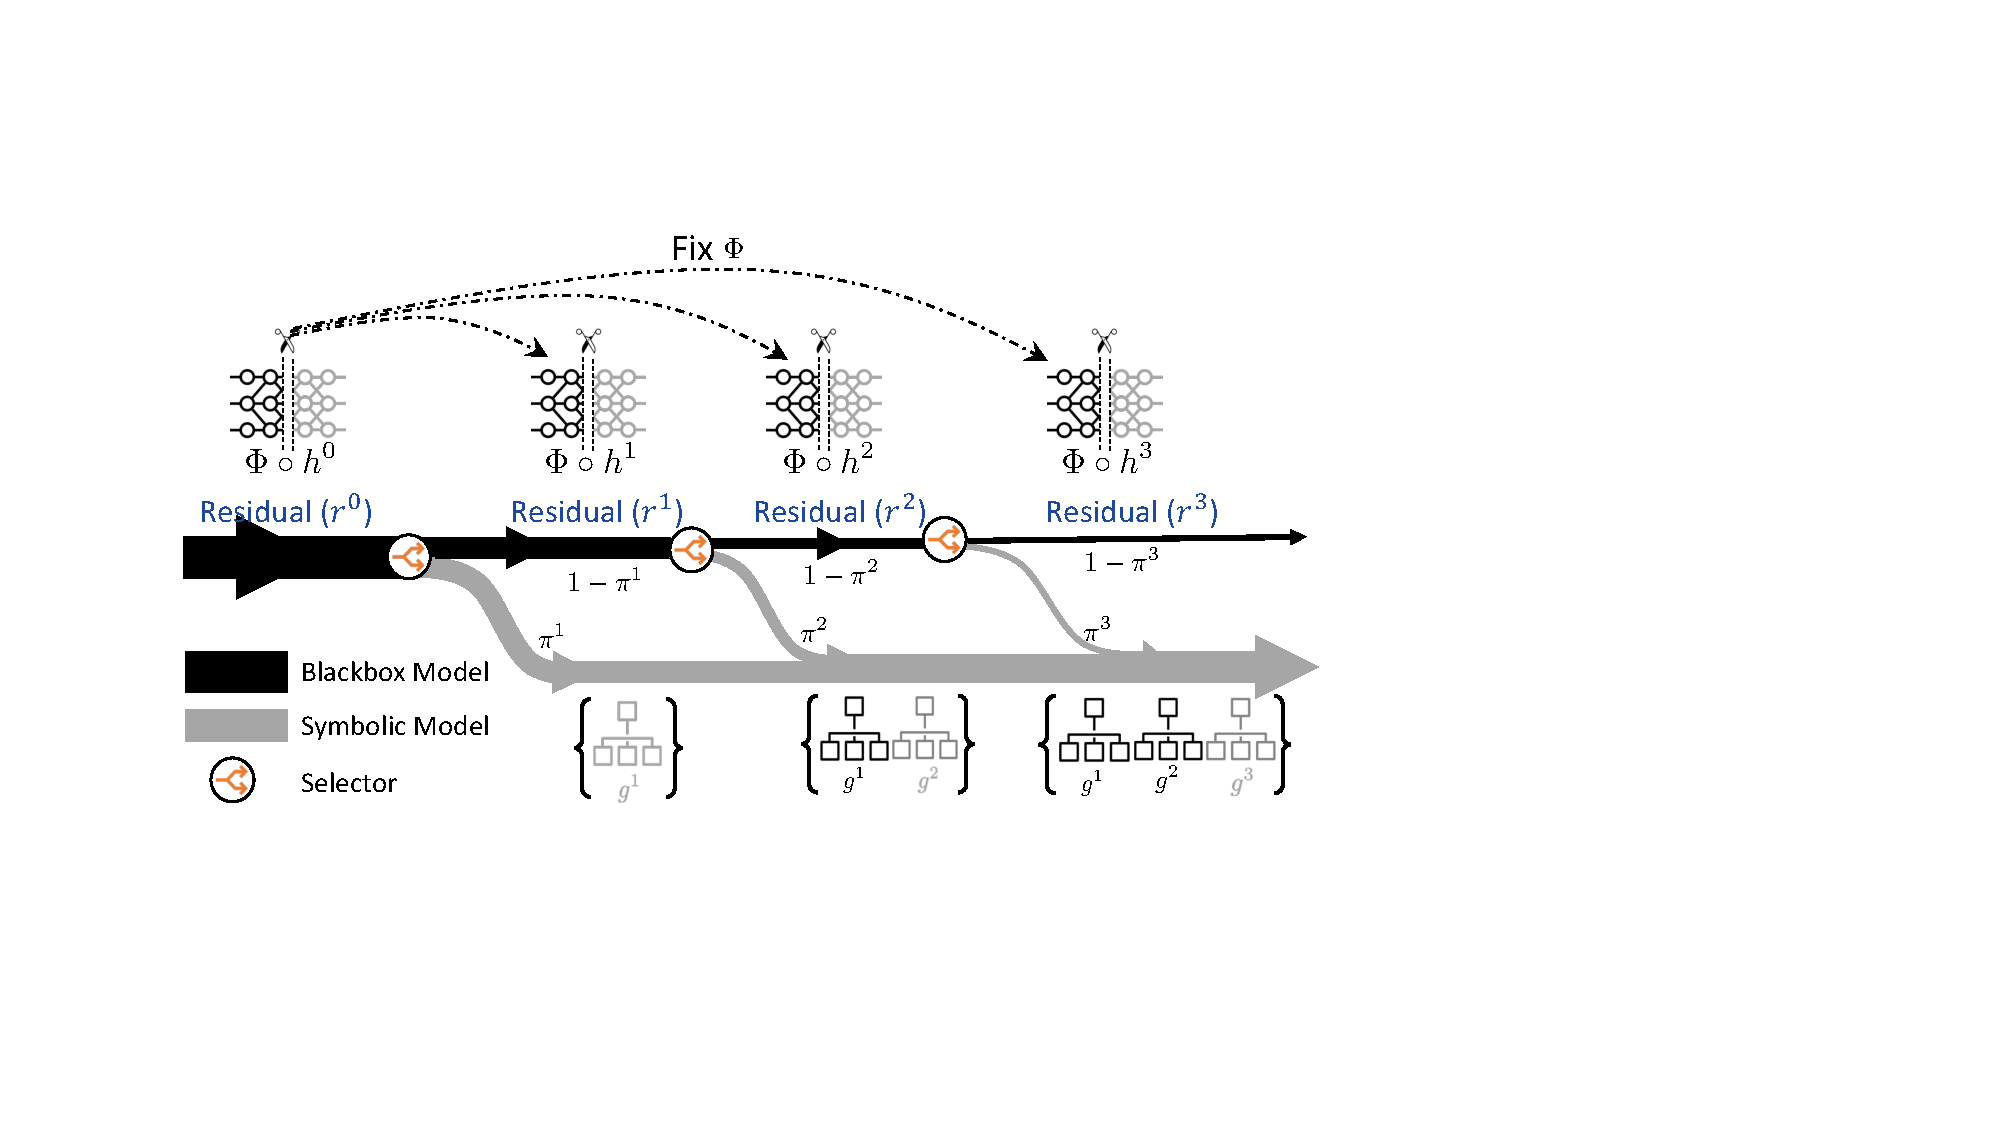
\includegraphics[width=\columnwidth]{figures/main/schematic.pdf}
\vskip -3pt
\caption{Schematic view of \emph{route, interpret} and \emph{repeat}. At iteration $k$, the selector \emph{routes} each sample either towards the interpretable model $g^k$ (to \emph{interpret}) with probability $\pi^k(.)$ or the residual $r^k = f^{k-1} - g^k$ with probability $1-\pi^k(.)$ (to \emph{repeat} in the further iterations). $f^{k-1}$ is the Blackbox of the $(k-1)^{th}$ iteration. $g^k$ generates FOL-based explanations for the samples it covers. Otherwise, the selector routes through the next step until it either goes through a subsequent interpretable model or reaches the last residual. Also, components in black and grey indicate the fixed and trainable modules in our model respectively. }
\label{fig:Schematic} 
\vskip -0.1in
\end{figure}

\subsubsection{The selector function}
As the first step of our method, the selector $\pi^k$ \emph{routes} the $j^{th}$ sample through the interpretable model $g^k$ or residual $r^k$ with probability $\displaystyle \pi^k(\boldsymbol{c_j})$ and $\displaystyle 1 - \pi^k(\boldsymbol{c_j})$ respectively, where $k$ $\in [0,K]$, with $K$ being the number of iterations.
We define the empirical coverage of the $\displaystyle k^{th}$ iteration as $\vspace{-0.08pt} \zeta(\pi^k) = \frac{1}{m}\sum_{j = 1} ^ m \pi^k(\boldsymbol{c_j}) \vspace{-0.081pt}$, the empirical mean of the samples selected by the selector for the associated interpretable model $\displaystyle g^k$, with $\displaystyle m$ being the total number of samples in the training set. Thus, the entire selective risk is:

\vskip -7.5pt
\begin{equation}
\label{equ: emp_risk}
\mathcal{R}^k(\displaystyle \pi^k, \displaystyle g^k) = \frac{\frac{1}{m}\sum_{j=1}^m\mathcal{L}_{(g^k, \pi^k)}^k\big(\boldsymbol{x_j}, \boldsymbol{c_j}\big)}{\zeta(\pi^k)} ,
\end{equation}
\vskip 2pt

where $\mathcal{L}_{(g^k, \pi^k)}^k$ is the optimization loss used to learn $\displaystyle g^k$ and $\displaystyle \pi^k$ together, discussed in section \ref{ns-optimization}. For a given coverage of $\displaystyle \tau^k \in (0, 1]$, we solve the following optimization problem:

\vskip -7.5pt
\begin{align}
\label{equ: optimization_g}
\theta_{s^k}^*, \theta_{g^k}^* = & \operatorname*{arg\,min}_{\theta_{s^k}, \theta_{g^k}} \mathcal{R}^k\Big(\pi^k(.; \theta_{s^k}), \displaystyle g^k(.; \theta_{g^k}) \Big) \nonumber \\ 
&\text{s.t.} ~~~ \zeta\big(\pi^k(.; \theta_{s^k})\big) \geq \tau^k,
\end{align}
\vskip 2pt

where $\theta_{s^k}^*, \theta_{g^k}^*$ are the optimal parameters at iteration $k$ for the selector $\pi^k$ and the interpretable model $g^k$ respectively. In this work, $\pi$s' of different iterations are neural networks with sigmoid activation. At inference time, the selector routes the $j^{th}$ sample with concept vector $\boldsymbol{c_j}$ to $\displaystyle g^k$ if and only if $\pi^k(\boldsymbol{c}_j)\geq 0.5$ for $k \in [0,K]$.

\subsubsection{Neuro-Symbolic interpretable models}
\label{ns-optimization}
In this stage, we design interpretable model $\displaystyle g^k$ of $k^{th}$ iteration  to \emph{interpret} the Blackbox $\displaystyle f^{k - 1}$ from the previous $(k-1)^{th}$ iteration by optimizing the following loss function:
\begin{equation}
\label{equ: g_k}
\resizebox{0.47\textwidth}{!}{$
\mathcal{L}_{(g^k, \pi^k)}^k\big(\boldsymbol{x_j}, \boldsymbol{c_j}\big) = \underbrace{\mystrut{2.6ex}\ell\Big(f^{k - 1}(\boldsymbol{x_j}), g^k(\boldsymbol{c_j})\Big)\pi^k(c_j) }_{\substack{\text{trainable component} \\ \text{for current iteration $k$}}}\underbrace{\prod_{i=1} ^{k - 1}\big(1 - \pi^i(\boldsymbol{c_j})\big)}_{\substack{\text{fixed component trained} \\ \text{in the previous iterations}}},
$}
\end{equation}

where the term $\pi^k(\boldsymbol{c_j})\prod_{i=1} ^{k - 1}\big(1 - \pi^i(\boldsymbol{c_j}) \big)$ denotes the probability of $j^{th}$ sample being routed through the interpretable model $g^k$. It is the probability of the sample going through the residuals for all the previous iterations from $0$ through $k-1$ (\ie $\prod_{i=1} ^{k - 1}\big(1 - \pi^i(\boldsymbol{c_j}) \big)$\big) times the probability of going through the interpretable model at iteration $k$ \big(\ie $\pi^k(\boldsymbol{c_j})$\big). 
Refer to Figure~\ref{fig:Schematic} for an illustration. We learn $\pi^1, \dots \pi^{k - 1}$ in the prior iterations and are not trainable at iteration $k$. As each interpretable model $g^k$ specializes in explaining a specific subset of samples (denoted by coverage $\tau$), we refer to it as an \emph{expert}. We use SelectiveNet's ~\cite{geifman2019selectivenet}  optimization method to optimize equation \ref{equ: optimization_g} since selectors need a rejection mechanism to route samples through residuals. Appendix \ref{app:loss} details the optimization procedure in equation \ref{equ: g_k}. We refer to the interpretable experts of all the iterations as a ``Mixture of Interpretable Experts'' (MoIE) cumulatively after training. Furthermore, we utilize Entropy-based linear layer neural network (ELL)~\cite{barbiero2022entropy} as the interpretable symbolic model $g$ to construct First Order Logic (FOL) explanations of a given prediction.

\subsubsection{The Residuals}
The last step is to \emph{repeat} with the residual $r^k$, as $\displaystyle r^k(\boldsymbol{x_j},\boldsymbol{c_j}) = f^{k - 1}(\boldsymbol{x_j}) - g^k(\boldsymbol{c_j})$.
We train $f^k = h^k\big(\Phi(.)\big)$ to approximate the residual $r^k$, creating a new Blackbox $f^k$ for the next iteration $(k+1$). This step is necessary to specialize $\displaystyle f^k$ over samples not covered by $g^k$. Optimizing the following loss function yields $\displaystyle f^k$ for the $\displaystyle k^{th}$ iteration:
\begin{equation}
\label{equ: residual}
\mathcal{L}_f^k(\boldsymbol{x_j}, \boldsymbol{c_j}) = \underbrace{\mystrut{2.6ex}\ell\big(r^k(\boldsymbol{x_j}, \boldsymbol{c_j}), f^k(\boldsymbol{x_j})\big)}_{\substack{\text{trainable component} \\ \text{for iteration $k$}}} \underbrace{\mystrut{2.6ex}\prod_{i=1} ^{k}\big(1 - \pi^i(\boldsymbol{c_j})\big)}_{\substack{\text{non-trainable component} \\ \text{for iteration $k$}}} 
\end{equation}

% \underbrace{\mystrut{2.6ex}\ell\big(f^{k - 1}(\boldsymbol{x_j}), g^k(\boldsymbol{c_j})\big)\pi^k(c_j) }_{\substack{\text{trainable component} \\ \text{from current iteration}}}
Notice that we fix the embedding $\displaystyle \Phi(.)$ for all the iterations. Due to computational overhead, we only finetune the last few layers of the Blackbox ($h^k$) to train $f^k$.
At the final iteration $K$, our method produces a MoIE and a Residual, explaining the interpretable and uninterpretable components of the initial Blackbox $f^0$, respectively. Appendix \ref{app:algo} describes the training procedure of our model, the extraction of FOL and the architecture of our model at inference.


\textbf{Selecting number of iterations $K$:} We follow two principles to select the number of iterations $K$ as a stopping criterion: 1) Each expert should have enough data to be trained reliably (
coverage $\zeta^k$). If an expert covers insufficient samples, we stop the process. 2) If the final residual ($r^K$) underperforms a threshold, it is not reliable to distill from the Blackbox. We stop the procedure to ensure the overall accuracy is maintained.
\label{sec:method}

\section{Experiments}
We perform experiments to show that MoIE-CXR 1) captures a diverse set of concepts, 2) does not compromise BB's performance, 3) covers ``harder'' instances with the residuals in later iterations resulting in their drop in performance, 4) is finetuned well to an unseen domain with minimal computation. 

\begin{figure*}[ht]
\begin{center}
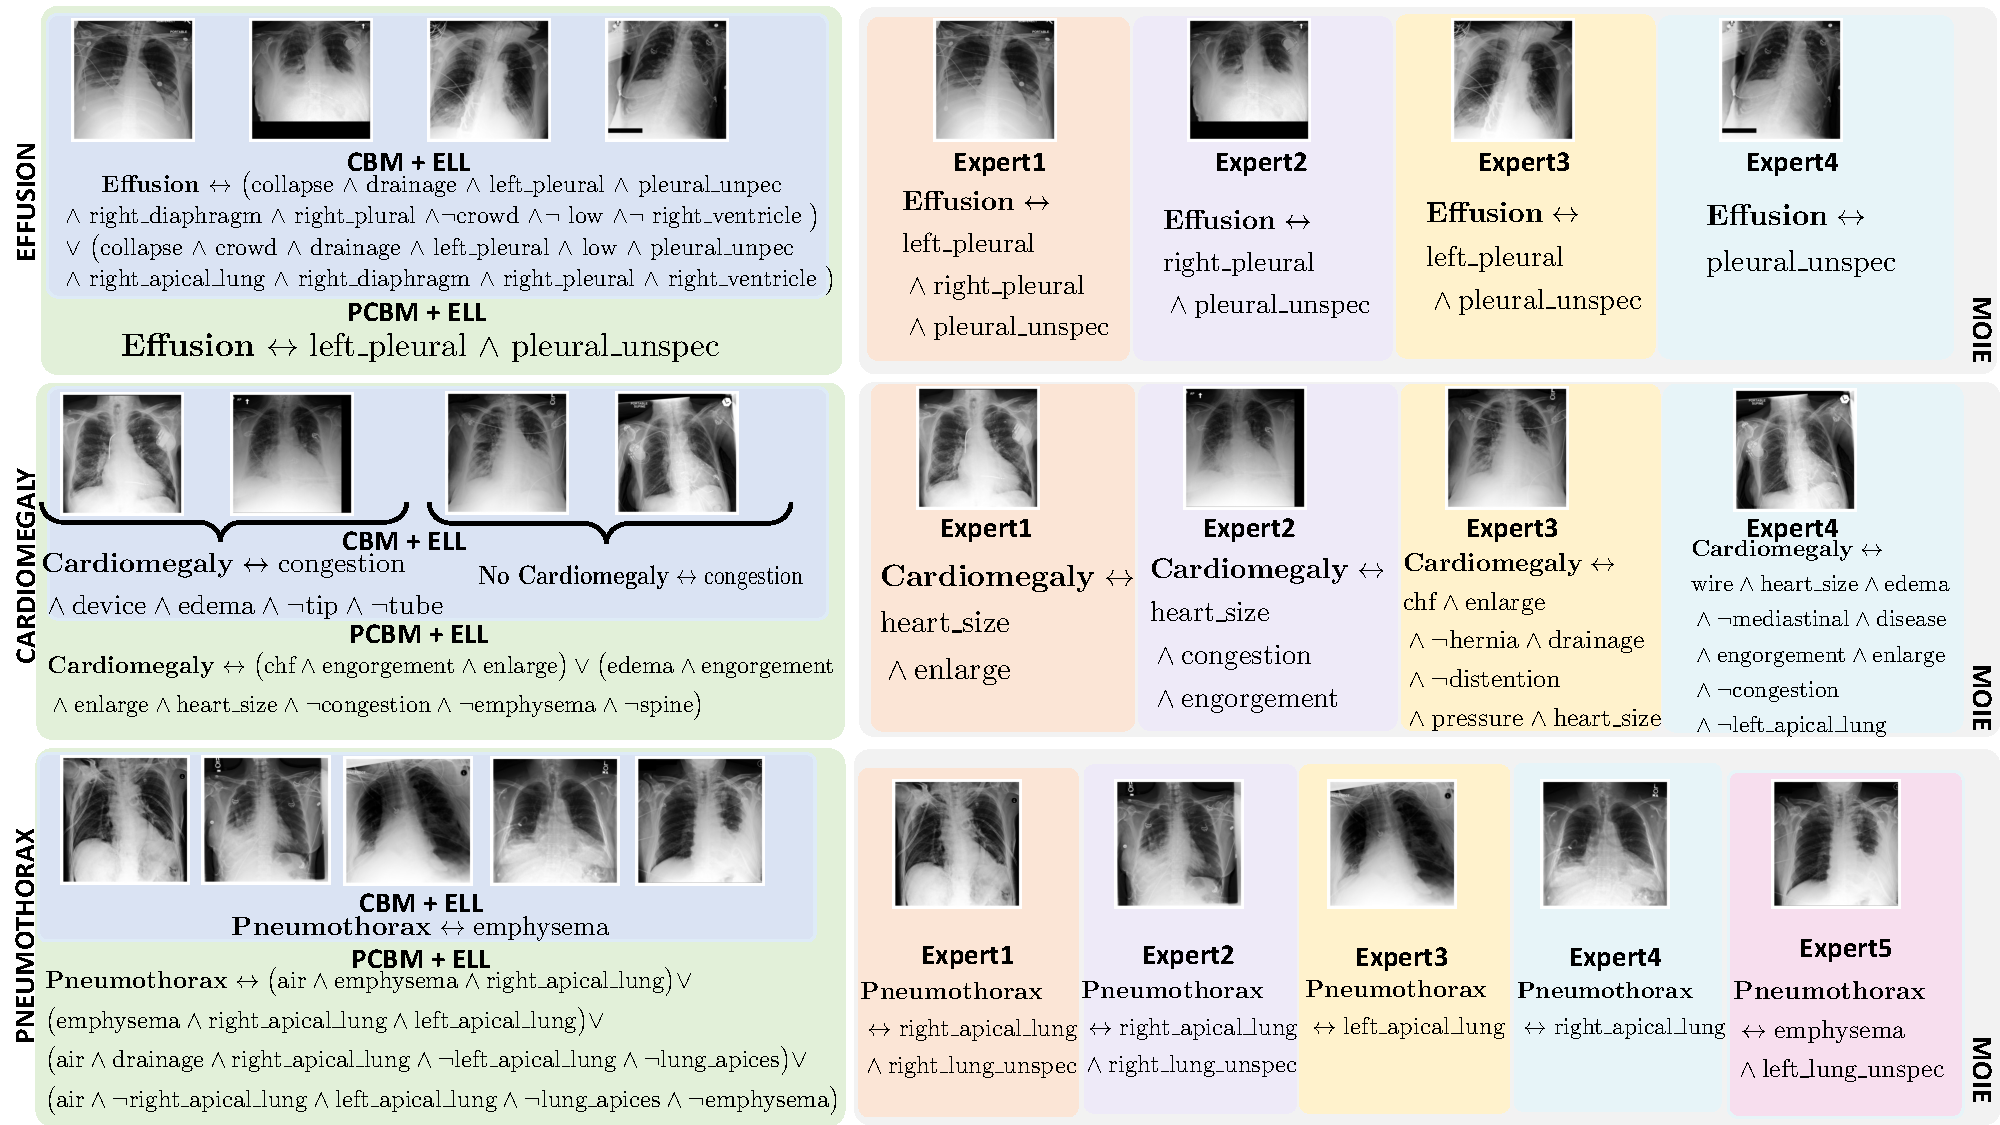
\includegraphics[width=\linewidth]{plots/main/Qual_main_up.pdf}
\caption{Qualitative comparison of MoIE-CXR discovered concepts with the baselines.}
\label{fig:qual}
\end{center}
\end{figure*}

\noindent \textbf{Experimental Details.} We evaluate our method using  220,763 frontal images from the MIMIC-CXR dataset \cite{12_johnsonmimic}. We use Densenet121 \cite{huang2017densely} as BB ($f^0$) to classify cardiomegaly, effusion, edema, pneumonia, and pneumothorax, considering each to be a separate binary classification problem. We obtain 107 anatomical and observation concepts from the RadGraph’s inference dataset~\cite{10_jain2021radgraph}, automatically generated by DYGIE++~\cite{23_wadden-etal-2019-entity}. We train BB following~\cite{yu2022anatomy}. To retrieve the concepts, we utilize until the $4^{th}$ Densenet block as feature extractor $\Phi$ and flatten the features to learn $t$. We use an 80\%-10\%-10\% train-validation-test split with no patient shared across splits. We use 4, 4, 5, 5, and 5 experts for cardiomegaly, pneumonia, effusion, pneumothorax, and edema. We employ ELL~\cite{barbiero2022entropy} as $g$. Further, we only include concepts as
input to $g$ if their validation auroc exceeds 0.7. Refer to Tab. 1 in the supplementary material for the hyperparameters. 
% We train the model on a single NVIDIA GPU-32G of memory. 
We stop until all the experts cover at least 90\% of the data cumulatively. \noindent \textbf{Baseline.} We compare our method with 1) end-to-end CEM~\cite{zarlenga2022concept}, 2) sequential CBM~\cite{koh2020concept}, and 3) PCBM~\cite{yuksekgonul2022post} baselines, comprising of two parts: a) concept predictor $\Phi: \mathcal{X} \rightarrow \mathcal{C}$, predicting concepts from images, with all the convolution blocks; and b) label predictor, $g: \mathcal{C} \rightarrow \mathcal{Y}$, predicting labels from the concepts. We create CBM + ELL and PCBM + ELL by replacing the standard classifier with the identical $g$ of MOIE-CXR to generate FOLs~\cite{barbiero2022entropy} for the baseline.
\label{sec:experiment}

\noindent \textbf{MoIE-CXR captures diverse explanations.}
Fig.~\ref{fig:qual} illustrates the FOL explanations. Recall that the experts ($g$) in MoIE-CXR and the baselines are ELLs~\cite{barbiero2022entropy}, attributing attention weights to each concept. A concept with high attention weight indicates its high predictive significance. With a single $g$, the baselines rank the concepts in accordance with the identical order of attention weights for all the samples in a class, yielding  a generic FOL for that class. In Fig.~\ref{fig:qual}, the baseline PCBM + ELL uses \emph{left\_pleural} and \emph{pleural\_unspec} to identify effusion for all four samples. MoIE-CXR deploys multiple experts, learning to specialize in distinct subsets of a class. So different interpretable models in MoIE assign different attention weights to capture instance-specific concepts unique to each subset. In Fig.~\ref{fig:qual} expert2 relies on \emph{right\_pleural} and \emph{pleural\_unspec}, but expert4 relies only on \emph{pleural\_unspec} to classify effusion. 
The results show that the learned experts can provide more precise explanations at the subject level using the concepts, increasing confidence and trust in clinical use. 
\label{sec:qual_analysis}

\begin{table*}[h]
\caption{MoIE-CXR does not compromize the performance of BB. We 
provide the mean and standard errors of AUROC over five random seeds. For MoIE-CXR, we also report the percentage of test set samples covered by all experts as ``\emph{Coverage}''. We boldfaced our results and BB.}
\begin{adjustbox}{max width=1\textwidth, center}
\begin{tabular}{lccccccccc}
\toprule
\textbf{Model} &
  Effusion &
  Cardiomegaly &
  Edema &
  Pneumonia &
  Pneumothorax
  \\
\midrule 
  \scriptsize{Blackbox (BB)} & 
  \scriptsize{$\boldsymbol{0.92}$} & 
  \scriptsize{$\boldsymbol{0.84}$} & 
  \scriptsize{$\boldsymbol{0.89}$} & 
  \scriptsize{$\boldsymbol{0.79}$} 
  & \scriptsize{$\boldsymbol{0.91}$}
  \\
\midrule
\scriptsize{\textbf{INTERPRETABLE BY DESIGN}} \\
\scriptsize{CEM}~\cite{zarlenga2022concept} &
\scriptsize{$0.83_{\pm 1\mathrm{e}{-4}}$} &
\scriptsize{$0.75_{\pm 1\mathrm{e}{-4}}$} &
\scriptsize{$0.77_{\pm 2\mathrm{e}{-4}}$} &
\scriptsize{$0.62_{\pm 4\mathrm{e}{-4}}$} &
\scriptsize{$0.76_{\pm 3\mathrm{e}{-4}}$} &
\\
\scriptsize{CBM (Sequential)}~\cite{koh2020concept}  &  
\scriptsize{$0.78_{\pm 1\mathrm{e}{-4}}$} &
\scriptsize{$0.72_{\pm 1\mathrm{e}{-4}}$} &
\scriptsize{$0.77_{\pm 5\mathrm{e}{-4}}$} &
\scriptsize{$0.60_{\pm 1\mathrm{e}{-3}}$} &
\scriptsize{$0.75_{\pm 6\mathrm{e}{-4}}$} &
\\
\scriptsize{CBM + ELL}~\cite{koh2020concept, barbiero2022entropy}    &
\scriptsize{$0.81_{\pm 1\mathrm{e}{-4}}$} &
\scriptsize{$0.72_{\pm 1\mathrm{e}{-4}}$} &
\scriptsize{$0.79_{\pm 5\mathrm{e}{-4}}$} &
\scriptsize{$0.62_{\pm 8\mathrm{e}{-4}}$} &
\scriptsize{$0.75_{\pm 6\mathrm{e}{-4}}$} &
\\

\midrule
\scriptsize{\textbf{POSTHOC}} \\
\scriptsize{PCBM}~\cite{yuksekgonul2022post} & 
\scriptsize{$0.88_{\pm 1\mathrm{e}{-4}}$} & 
\scriptsize{$0.81_{\pm 1\mathrm{e}{-4}}$} & 
\scriptsize{$0.82_{\pm 1\mathrm{e}{-4}}$} &
\scriptsize{$0.72_{\pm 1\mathrm{e}{-4}}$} &
\scriptsize{$0.85_{\pm 7\mathrm{e}{-4}}$} &
 \\ 
\scriptsize{PCBM-h}~\cite{yuksekgonul2022post} &
\scriptsize{$0.90_{\pm 1\mathrm{e}{-4}}$} &
\scriptsize{$0.83_{\pm 1\mathrm{e}{-4}}$} & 
\scriptsize{$0.85_{\pm 1\mathrm{e}{-4}}$} &
\scriptsize{$0.77_{\pm 1\mathrm{e}{-4}}$} &
\scriptsize{$0.89_{\pm 7\mathrm{e}{-4}}$} &
\\ 
\scriptsize{PCBM + ELL}~\cite{yuksekgonul2022post, barbiero2022entropy} &
\scriptsize{$0.90_{\pm 1\mathrm{e}{-4}}$} &
\scriptsize{$0.82_{\pm 1\mathrm{e}{-4}}$} &
\scriptsize{$0.85_{\pm 1\mathrm{e}{-4}}$} &
\scriptsize{$0.75_{\pm 1\mathrm{e}{-4}}$} &
\scriptsize{$0.85_{\pm 6\mathrm{e}{-4}}$} &
\\
\scriptsize{PCBM-h + ELL}~\cite{yuksekgonul2022post, barbiero2022entropy} &
\scriptsize{$0.91_{\pm 1\mathrm{e}{-4}}$} &
\scriptsize{$0.83_{\pm 1\mathrm{e}{-4}}$} & 
\scriptsize{$0.87_{\pm 1\mathrm{e}{-4}}$} &
\scriptsize{$0.77_{\pm 1\mathrm{e}{-4}}$} &
\scriptsize{$0.90_{\pm 1\mathrm{e}{-4}}$} &
\\
 
\midrule
\scriptsize{\textbf{OURS}} \\
\scriptsize{MoIE-CXR $^{\text{(Coverage)}}$} & 
\scriptsize{$\boldsymbol{0.93^\textbf{\emph{(0.90)}}_{\pm 1\mathrm{e}{-4}}}$} &
\scriptsize{$\boldsymbol{0.85^\textbf{\emph{(0.96)}}_{\pm 1\mathrm{e}{-4}}}$} &
\scriptsize{$\boldsymbol{0.91^\textbf{\emph{(0.92)}}_{\pm 1\mathrm{e}{-4}}}$} &
\scriptsize{$\boldsymbol{0.80^\textbf{\emph{(0.97)}}_{\pm 1\mathrm{e}{-4}}}$} &
\scriptsize{$\boldsymbol{0.91^\textbf{\emph{(0.93)}}_{\pm 2\mathrm{e}{-4}}}$} &
\\ 

\scriptsize{MoIE-CXR+R} & 
\scriptsize{$\boldsymbol{0.91_{\pm 1\mathrm{e}{-4}}}$} &
\scriptsize{$\boldsymbol{0.82_{\pm 1\mathrm{e}{-4}}}$} &
\scriptsize{$\boldsymbol{0.88_{\pm 1\mathrm{e}{-4}}}$} &
\scriptsize{$\boldsymbol{0.78_{\pm 1\mathrm{e}{-4}}}$} &
\scriptsize{$\boldsymbol{0.90_{\pm 2\mathrm{e}{-4}}}$}
\\ 
\bottomrule
\end{tabular}
\end{adjustbox}
\label{tab:performance}
\end{table*}

\noindent \textbf{MoIE-CXR does not compromise BB's performance.}
\noindent \textbf{Analysing MoIE-CXR:} Tab.~\ref{tab:performance} shows that MoIE-CXR outperforms other models, including BB. Recall that MoIE-CXR refers to the mixture of all interpretable experts, excluding any residuals. As MoIE-CXR specializes in various subsets of data, it effectively discovers sample-specific classifying concepts and achieves superior performance.
In general, MoIE-CXR exceeds the interpretable-by-design baselines (CEM, CBM, and CBM + ELL) by a fair margin (on average, at least $\sim 10\% \uparrow$), especially for pneumonia and pneumothorax where the number of samples with the disease is significantly less ($\sim 750/24000$ in the testset).
\noindent\textbf{Analysing MoIE-CXR+R:}
 To compare the performance on the entire dataset, we additionally report MoIE-CXR+R, the mixture of interpretable experts with the final residual in Tab.\ref{tab:performance}. MoIE-CXR+R outperforms the interpretable-by-design models and yields comparable performance as BB. The residualized PCBM baseline, \ie PCBM-h, performs similarly to MoIE-CXR+R.
 PCBM-h rectifies the interpretable PCBM's mistakes by learning the residual with the complete dataset to resemble BB's performance. However, the experts and the final residual approximate the interpretable and uninterpretable fractions of BB, respectively. In each iteration, the residual focuses on the samples not covered by the respective expert to create BB for the next iteration and likewise. As a result, the final residual in MoIE-CXR+R covers the "hardest" examples, reducing its overall performance relative to MoIE-CXR. 
\label{sec:quant_analysis}


\begin{figure*}[t]
\begin{center}
\centerline{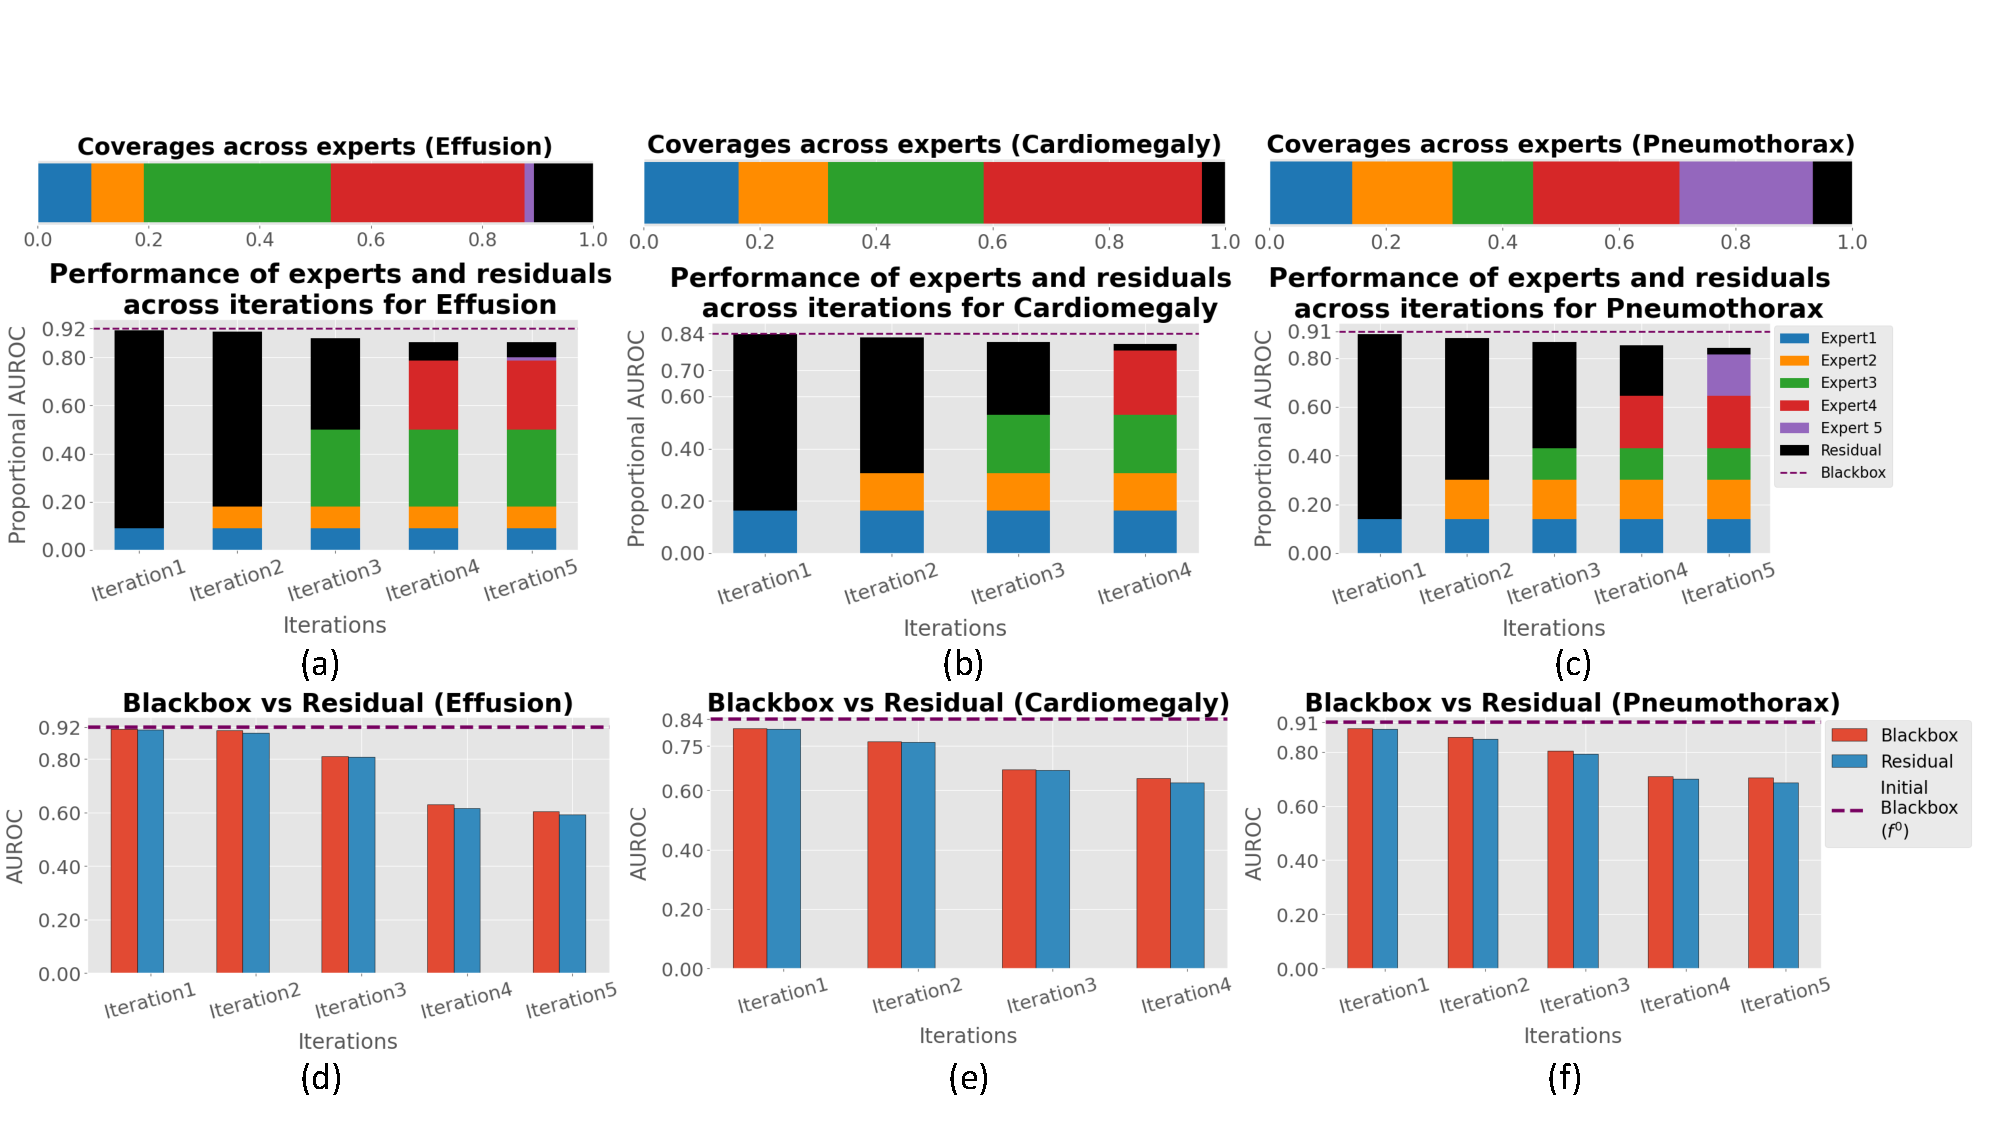
\includegraphics[width=\linewidth]{plots/main/Experts.pdf}}
\caption{Performance of experts and residuals across iterations. 
\textbf{(a-c):} Coverage and proportional AUROC of the experts and residuals.
\textbf{(d-f):} Routing the samples covered by MoIE-CXR to the initial $f^0$, we compare the performance of the residuals with $f^0$.
}
\label{fig:expert_performance_cv_vit}
\end{center}
\end{figure*}

\noindent \textbf{Identification of harder samples by successive residuals.}
Fig.~\ref{fig:expert_performance_cv_vit} (a-c) reports the proportional AUROC of the experts and the residuals per iteration. The proportional AUROC is the AUROC of that model times the empirical coverage, $\zeta^k$, the mean of the samples routed to the model by the respective selector ($\pi^k$).
According to Fig.~\ref{fig:expert_performance_cv_vit}a in iteration 1, the residual (black bar) contributes more to the proportional AUROC than the expert1 (blue bar) for effusion with both achieving a cumulative proportional AUROC~$\sim$ 0.92. All the final experts collectively extract the entire interpretable component from BB $f^0$ in the final iteration, resulting in their more significant contribution to the cumulative performance. In subsequent iterations, the proportional AUROC decreases as the experts are distilled from the BB of the previous iteration. The BB is derived from the residual that performs progressively worse with each iteration. The residual of the final iteration covers the ``hardest'' samples. Tracing these samples back to the original BB $f^0$, $f^0$ underperforms on these samples (Fig.~\ref{fig:expert_performance_cv_vit} (d-f)) as the residual.



\label{sec:residual_performance}

\begin{figure*}[t]
\vskip 0.2in
\begin{center}
\centerline{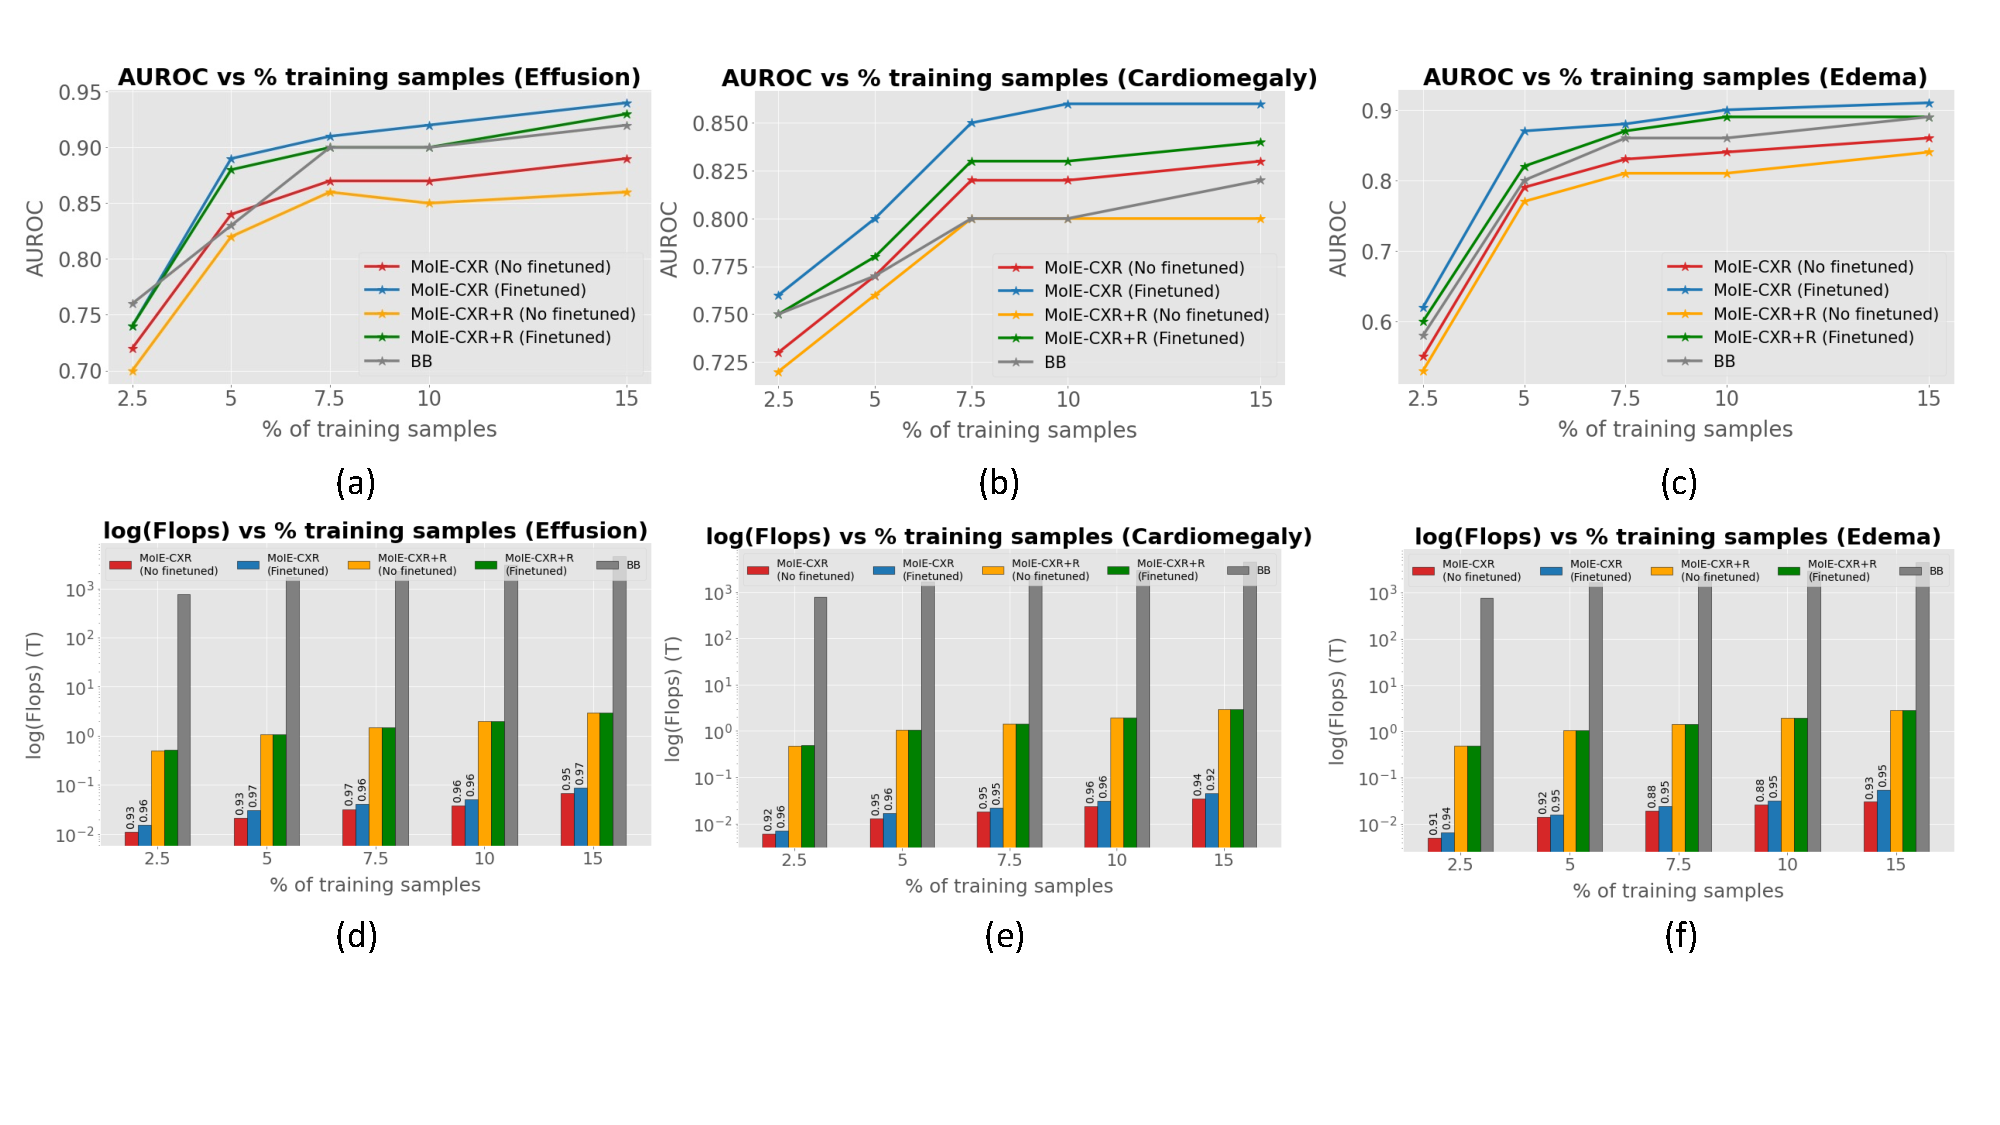
\includegraphics[width=\linewidth]{plots/main/Domain_genelization.pdf}}
\caption{Transfering the first 3 experts of MoIE-CXR trained on MIMIC-CXR to Stanford-CXR. With varying \% of training samples of Stanford CXR, \textbf{(a-c):}  reports AUROC of the test sets, \textbf{(d-g)} reports computation costs in terms of $\log\text{(Flops) (T)}$.
We report the coverages in Stanford-CXR on top of the ``finetuned'' and ``No finetuned'' variants of MoIE-CXR (red and blue bars) in \textbf{(d-g)}.
% The ``No finetuned'' variant of MoIE-CXR represents the model obtained only by finetuning selectors ($\pi$), not the experts ($g$). Similarly, the ``Finetuned'' MoIE-CXR represents the model obtained by jointly finetuning $\pi$ and $g$ for 5 epochs.
}
\label{fig:domain_generelization}
\end{center}
\end{figure*}

\noindent \textbf{Applying MoIE-CXR to the unseen domain.} In this experiment, we utilize Algo.~\ref{algo: domain_transfer} to transfer MoIE-CXR trained on MIMIC-CXR dataset to Stanford Chexpert~\cite{irvin2019chexpert} dataset for the diseases -- effusion, cardiomegaly and edema. Using 2.5\%, 5\%, 7.5\%, 10\%, and 15 \% of training data from the Stanford Chexpert dataset, we employ two variants of MoIE-CXR where we (1) train only the selectors ($\pi$) without finetuning the experts ($g$) (``No finetuned'' variant of MoIE-CXR in Fig.~\ref{fig:domain_generelization}), and (2) finetune $\pi$ and $g$ jointly for only 5 epochs (``Finetuned'' variant of MoIE-CXR and MoIE-CXR + R in Fig.~\ref{fig:domain_generelization}). Finetuning $\pi$ is essential to route the samples of the target domain to the appropriate expert. As later experts cover the ``harder'' samples of MIMIC-CXR, we only transfer the experts of the first three iterations (refer to Fig.~\ref{fig:expert_performance_cv_vit}). To ensure a fair comparison, we finetune (both the feature extractor $\Phi$ and classifier $h^0$) BB: $f^0 = h^0 \circ \Phi$ of MIMIC-CXR with the same training data of Stanford Chexpert for 5 epochs. Throughout this experiment, we fix $\Phi$ while finetuning the final residual in MoIE+R as stated in Eq.~\ref{equ: residual}. Fig.~\ref{fig:domain_generelization} displays the performances of different models and the computation costs in terms of Flops. The Flops are calculated as, Flop of (forward propagation + backward propagation) $\times$ (total no. of batches) $\times$ (no of training epochs). The finetuned MoIE-CXR outperforms the finetuned BB (on average $\sim 5\% \uparrow$ for effusion and cardiomegaly).
As experts are simple models~\cite{barbiero2022entropy} and accept only low dimensional concept vectors compared to BB, the computational cost to train MoIE-CXR is significantly lower than that of BB (Fig.~\ref{fig:domain_generelization} (d-f)). Specifically, BB requires $\sim$ 776T flops to be finetuned on 2.5\% of the training data of Stanford CheXpert, whereas MoIE-CXR requires $\sim$ 0.0065T flops. As MoIE-CXR discovers the sample-specific domain-invariant concepts, it achieves such high performance with low computational cost than BB. 

\label{sec:domain_genralization}

\section{Conclusion}


This paper proposes a novel method to iteratively extract a mixture of interpretable models from a flexible Blackbox. The comprehensive experiments on various datasets demonstrate that our method 1) captures more meaningful instance-specific concepts with high completeness score than baselines without losing the performance of the Blackbox, 2) does not require explicit concept annotation, 3) identifies the ``harder'' samples using the residuals, 4) achieves significant performance gain than the baselines during test time interventions, 5) eliminate shortcuts effectively. In the future, we aim to apply our method to other modalities, such as text or video. Also, as in the prior work, MoIE-captured concepts may not reflect a causal effect. The assessment of causal concept effects necessitates estimating inter-concept interactions, which will be the subject of future research.
\label{sec:conclusion}

\section{Acknowledgement}
We would like to thank Mert Yuksekgonul of Stanford University for providing the code to construct the concept bank of Derm7pt for conducting the skin experiments. This work was partially supported by NIH Award Number 1R01HL141813-01 and the Pennsylvania Department of Health. We are grateful for the computational resources provided by Pittsburgh Super Computing grant number TG-ASC170024.


\label{sec:ack}

%\subsubsection{Acknowledgements} Please place your acknowledgments at
%the end of the paper, preceded by an unnumbered run-in heading (i.e.
%3rd-level heading).


%
% ---- Bibliography ----
%
% BibTeX users should specify bibliography style 'splncs04'.
% References will then be sorted and formatted in the correct style.
%
\bibliographystyle{splncs04}
\bibliography{main}

\appendix
\setcounter{table}{0}
\setcounter{figure}{0}
\renewcommand\thefigure{\thesection.\arabic{figure}}    
\renewcommand\thetable{\thesection.\arabic{table}}  
\newpage
\section*{Supplementary materials}
\begin{figure*}[h]
\begin{center}
\centerline{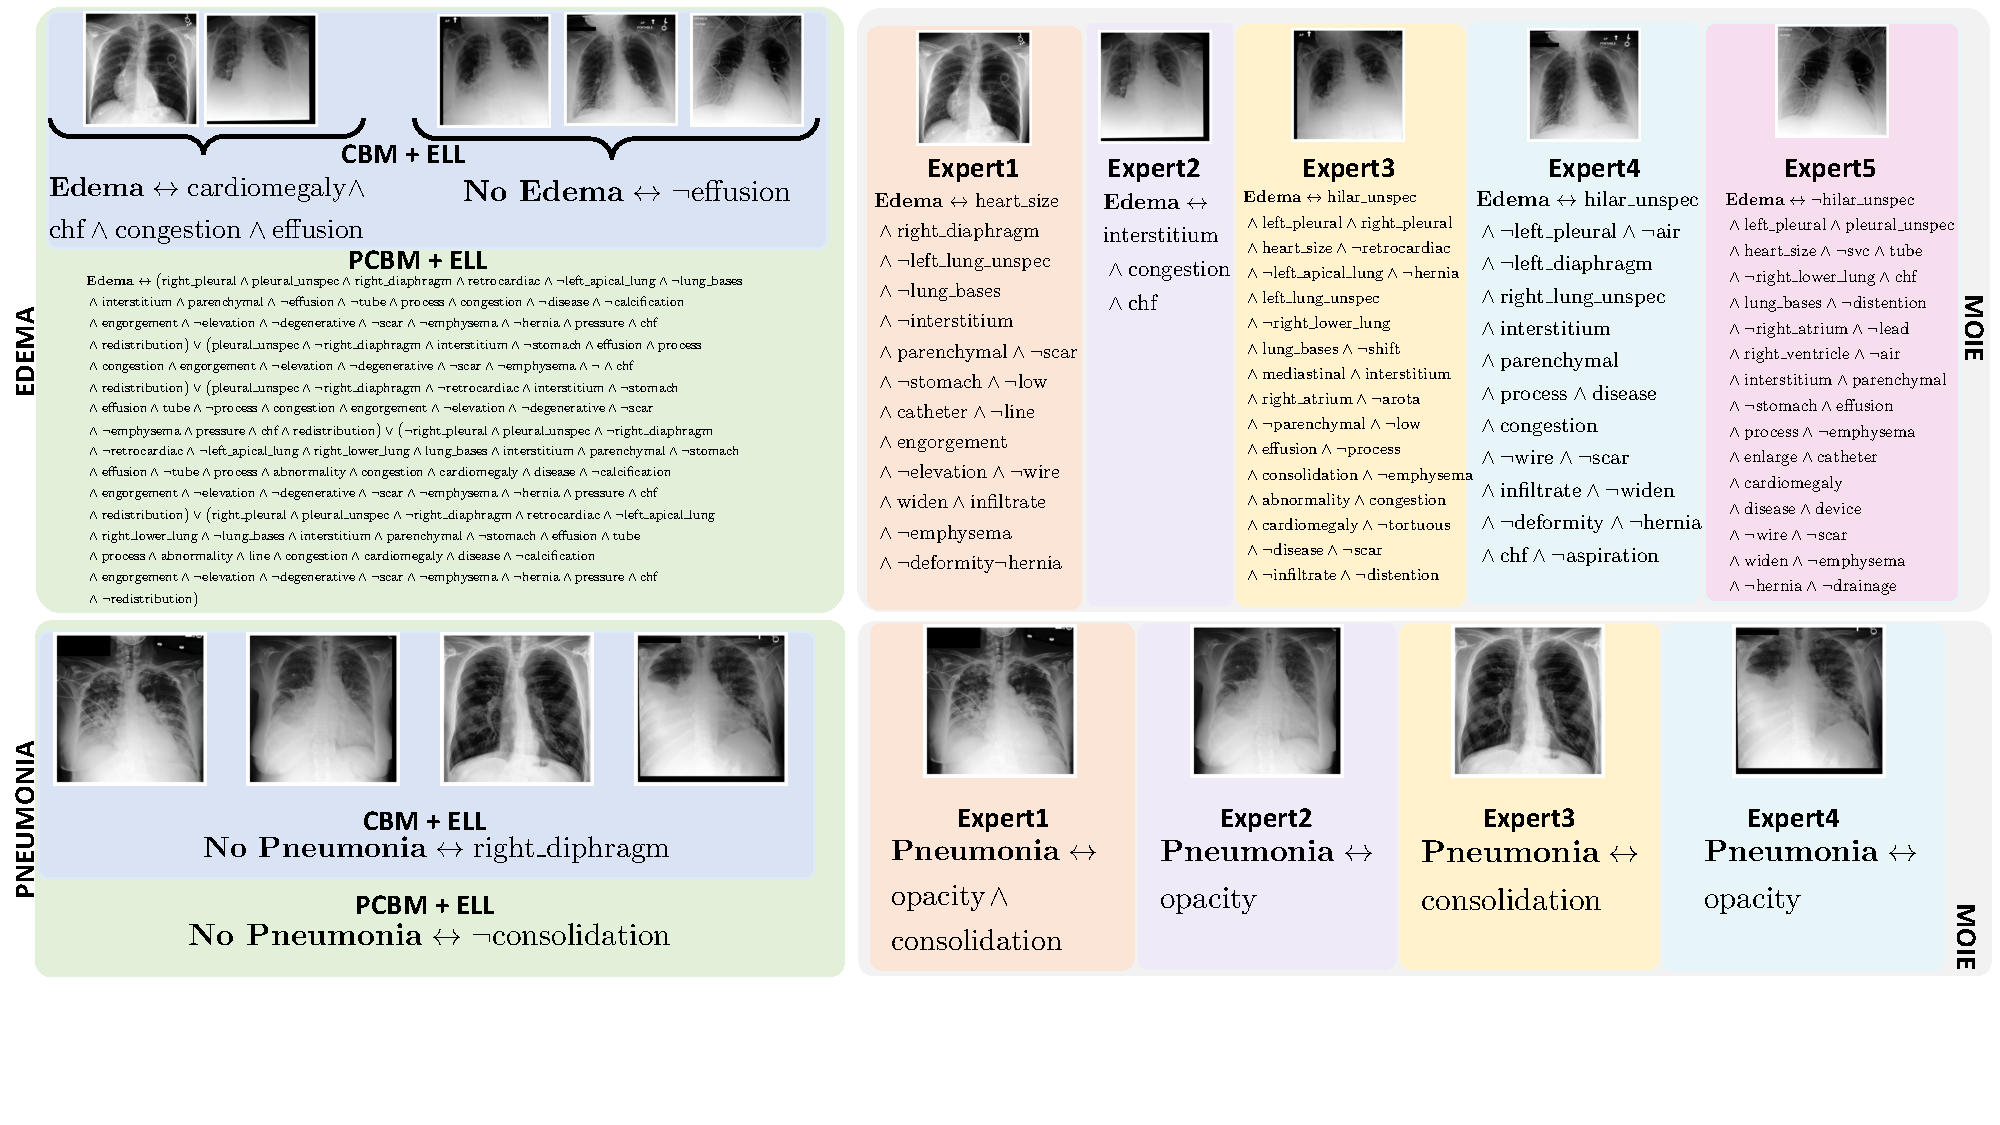
\includegraphics[width=\linewidth]{plots/supp/Supp_qual.pdf}}
\caption{Qualitative comparison of MoIE-CXR discovered concepts with the baseline for edema and pneumonia.}
\label{fig:expert_performance_cv_vit}
\end{center}
\end{figure*}

\begin{figure*}[h]
\begin{center}
\centerline{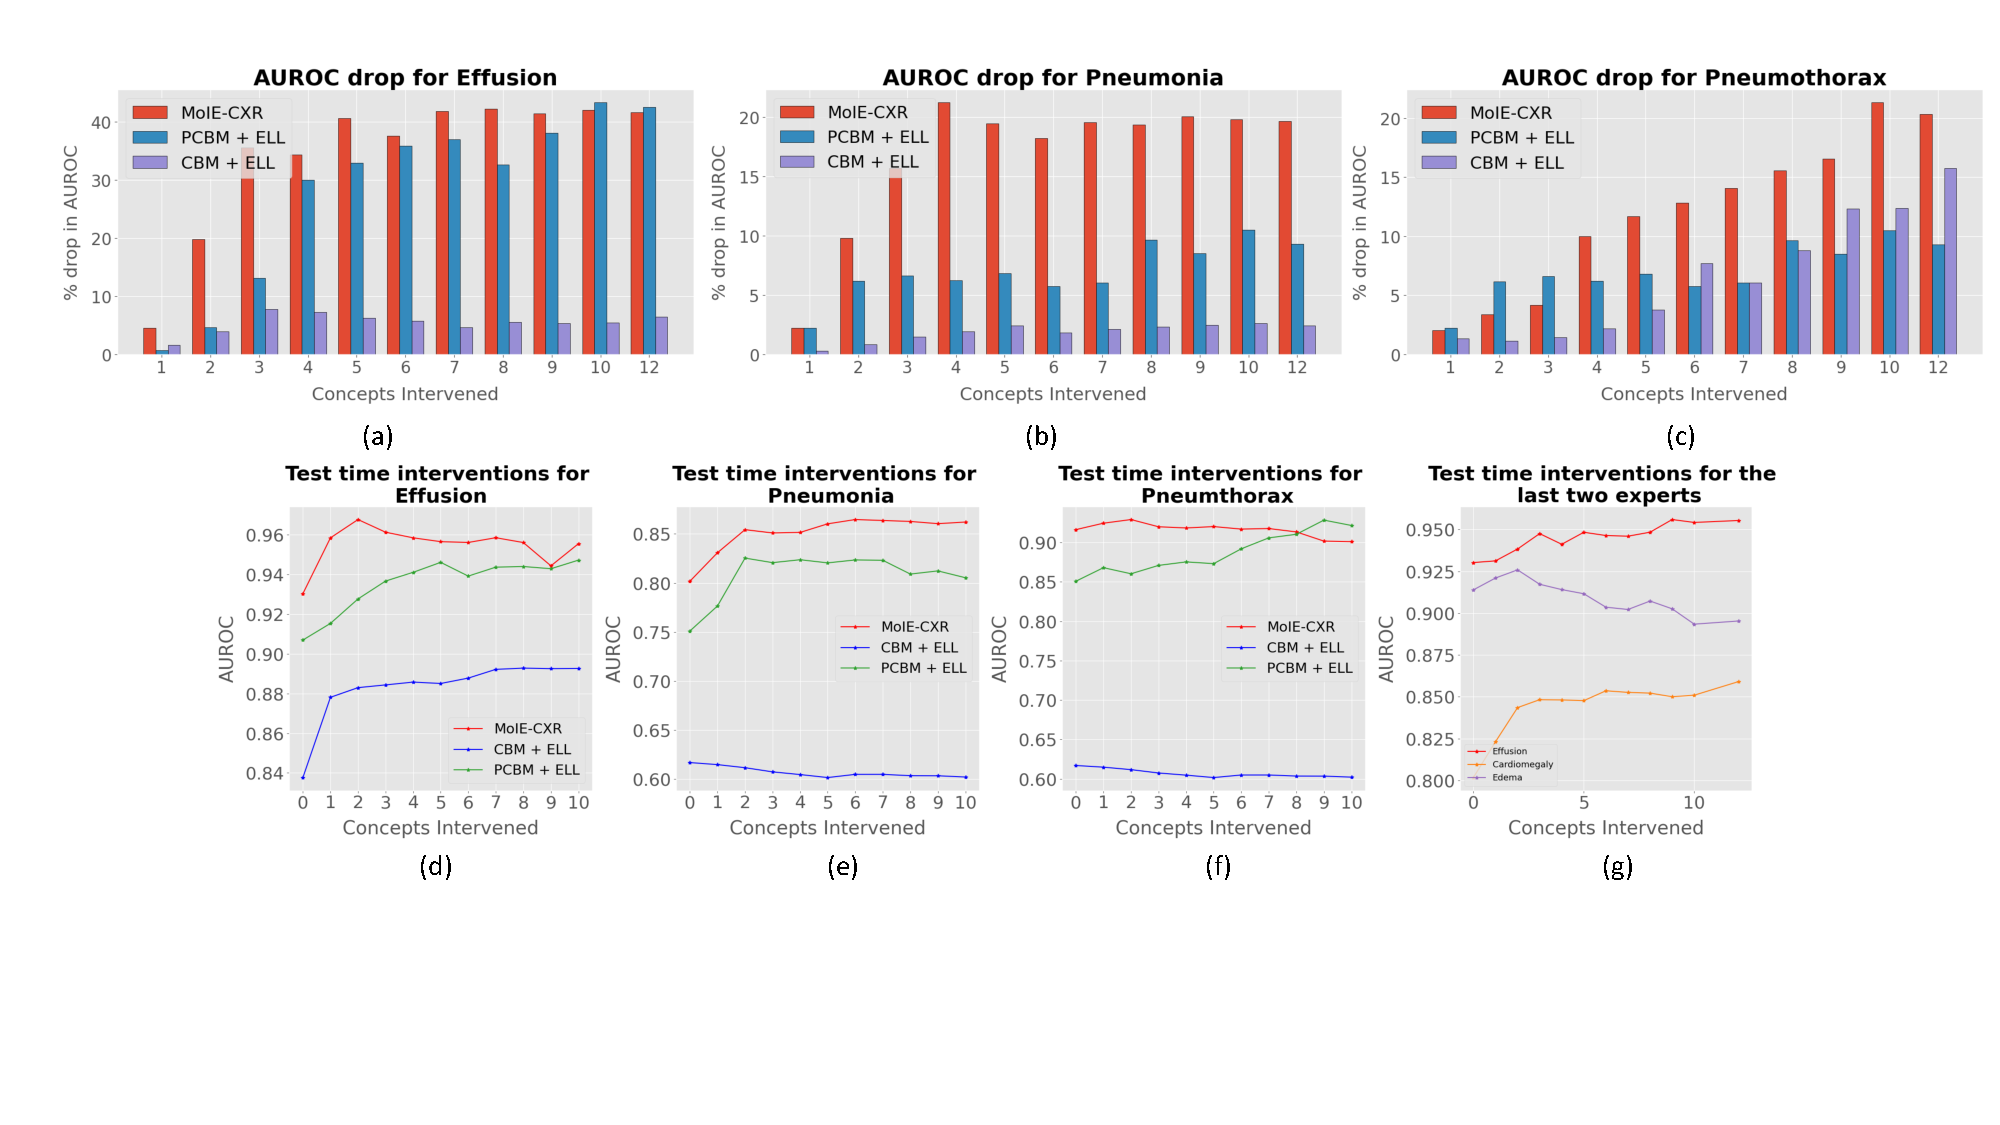
\includegraphics[width=\linewidth]{plots/supp/Supp_Quant_concepts.pdf}}
\caption{\textbf{(a-c):} Performance drop after zeroing out the concepts iteratively. The drop indicates the concepts to be more significant for prediction. \textbf{(d-g):} Test time interventions of concepts considering the ground truth concepts as an oracle on all samples (d-f), on the ``hard'' samples (g), covered by only the last two experts of MoIE-CXR.}
\label{fig:expert_performance_cv_vit}
\end{center}
\end{figure*}

\begin{figure*}[h]
\begin{center}
\centerline{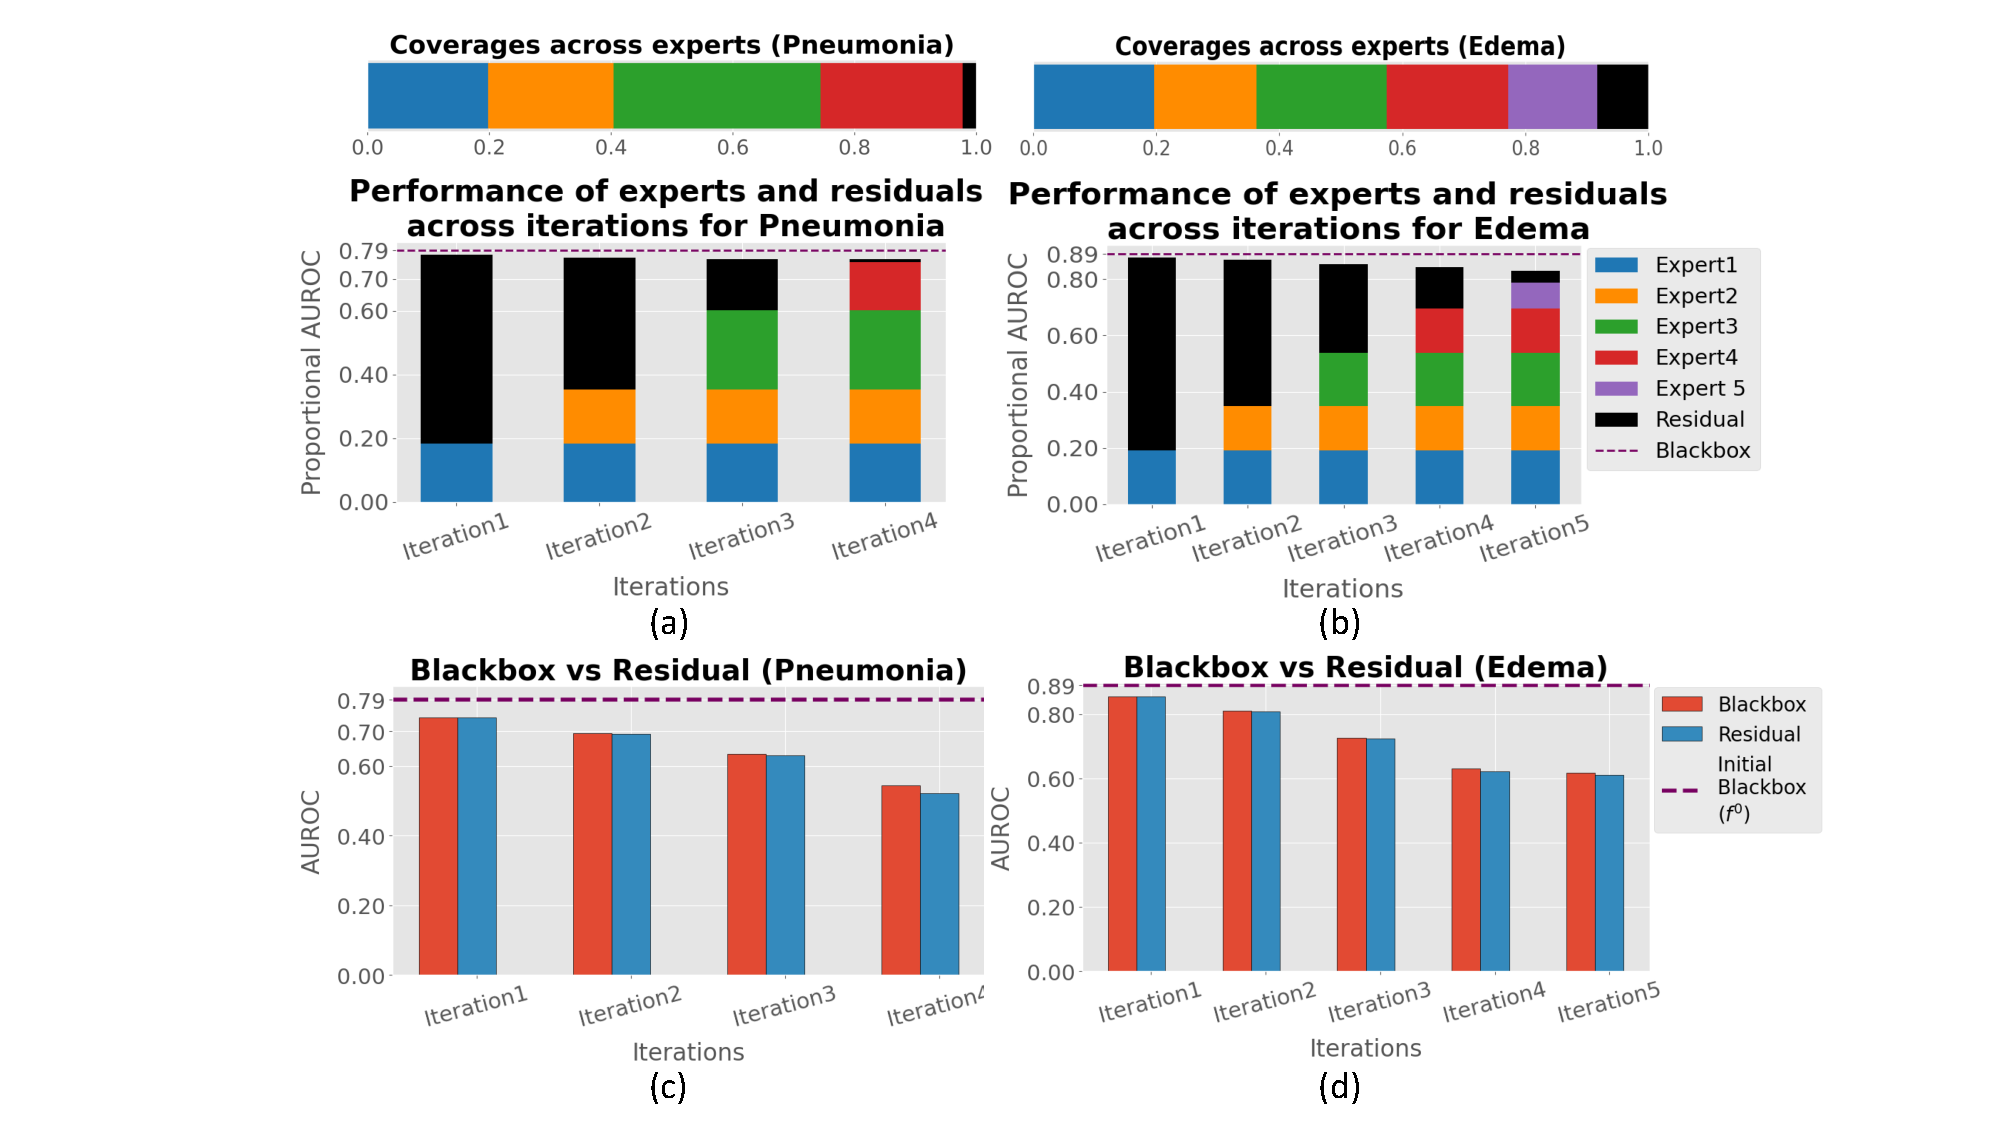
\includegraphics[width=\linewidth]{plots/supp/Supp_Experts.pdf}}
\caption{\textbf{(a-b)}: The performances of experts and residuals across iterations for pneumonia and edema. \textbf{(c-d)}: Performance comparison of the residuals and $f^0$ for the samples covered by the successive residuals.
}
\label{fig:expert_performance_cv_vit}
\end{center}
\end{figure*}

\begin{table}[H]
\caption{Hyperparameters of interpretable experts ($g$) for the dataset MIMIC-CXR.}
\label{tab:g_config_mimic_cxr}
\begin{center}
\begin{tabular}{l c c c c c }
\toprule 
    \thead{\textbf{Hyperparameter}} & 
    \thead{\textbf{Effusion}} & 
    \thead{\textbf{Cardiomegaly}} & 
    \thead{\textbf{Pneumothorax}} &
    \thead{\textbf{Pneumonia}} &
    \thead{\textbf{Edema}} \\
  
\midrule 
       Batch size & 1028 & 1028 & 1028 & 1028 & 1028   \\
       Learning rate & 0.01 & 0.01 & 0.01 & 0.01 & 0.01\\
       $\lambda_{lens}$ & 0.0001 & 0.0001 & 0.0001  & 0.0001 & 0.0001\\
       $\alpha_{KD}$ & 0.99 & 0.99 & 0.99 & 0.99 & 0.99 \\
       $T_{KD}$ & 20 & 20 & 20  & 20 & 20  \\
       hidden neurons & 30, 30 & 20, 20 & 20, 20 & 20, 20 & 20, 20 \\
       $\lambda_s$ & 96 & 1024 & 256 & 256 & 128   \\
       E-Lens ($T_{lens}$) & 7.6 & 7.6 & 10 & 10 & 7.6\\
       \# Expers ($T_{lens}$) & 5 & 4 & 5 & 4 & 5\\
\bottomrule
\end{tabular}
\end{center}
\end{table}

\end{document}

\label{sec:supplemental}
\end{document}
